\documentclass[11pt,a4paper,onecolumn,UTF8]{ctexart}
\usepackage{booktabs}
\usepackage{amsmath}
\usepackage{amsfonts}
\usepackage{amssymb}
\usepackage{amsthm}
\usepackage{mathrsfs} 
\usepackage{yhmath}
\usepackage{gensymb}
\usepackage{fancyvrb}
\usepackage{fancyhdr}
\usepackage[table]{xcolor}
\usepackage{float}
\usepackage{makecell}
\usepackage{booktabs}
\usepackage[colorlinks=true,urlcolor=black]{hyperref}
\usepackage{CJKfntef}
\usepackage[left=1.25in,right=1.25in,vmargin=1in]{geometry}
\usepackage{graphicx}
\usepackage{tikz}
\usepackage{pgfplots}
\usepackage{pgfplotstable}
\usepackage{subfig}
\usepackage{bbm}
\usepackage{braket}
\usepackage{fontawesome}
\allowdisplaybreaks[2]
\linespread{1.63}

\begin{document}
	\newcommand{\ui}{\mathbbm{i}}
	\newcommand{\ud}{\mathrm{d}}
	\newcommand{\ue}{\mathbbm{e}}
	\newcommand{\uT}{\mathrm{T}}
	
	
	\pagestyle{fancy}
	\fancyhead[L]{\textit{第一届离谱中学生物理竞赛}}
	\fancyhead[R]{\textit{The First Ridiculous Physics Olympiad}}
	
	{\large 离谱中学生物理竞赛命题组\,\,\,荣誉出品}\\[2ex]
	
	
	
	\thispagestyle{empty}
	\begin{center}
		\textbf{\LARGE{第一届\;}}\textbf{\huge{离谱}}\textbf{\LARGE{\;中学生物理竞赛}}\\[5ex]
		
		\textbf{\Huge{试题}}\\[10ex]
		
	\end{center}
	
	\begin{center}
		\Large{The First (1${}^{\text{st}}$)\;}\textbf{\LARGE{ RIDICULOUS }}\Large{\;Physics Olympiad}\\[5ex]
		
		\textbf{\huge{Problem Set}}\\[7ex]
		
		{\Large \textit{[Tempus edax, homo edacior.]}}\\[10ex]
		
	\end{center}
	
	{\normalfont 考试时间:\begin{minipage}{10ex}\textit{\color{white}这么多?}\\{\textit{12小时}\\3小时\\{\color{white}这么少?}}\end{minipage}\,\,\,\,\,\,试题总分:\begin{minipage}{8ex}{\textit{0分}\\320分}\end{minipage}\,\,\,\,\,\,命题人{\color{white}偶}:\begin{minipage}{20ex}{\color{white}你在找什么?}\\{\textit{berylliumcopper}\\berylliumcopper}\\{\color{white}B站同号}\end{minipage}\\[1ex]
	
	资料来源:berylliumcopper, HamiltonHuaji, yigo\\[1ex]
	
	特别感谢:Victor Hugo, Donald Ervin Knuth, Stephen Wolfram, Gabriel García Márquez\\[1ex]
	
	版本号:$(\ket{\uparrow\downarrow}-\ket{\downarrow\uparrow})/\sqrt{2}$\\[1ex]
	
	源码及PDF版本下载地址:\href{https://github.com/berylliumcopper/RPhO-1}{https://github.com/berylliumcopper/RPhO-1}
	
	转载请注明版权,禁止用于商业用途。}
	
	\newpage
	\thispagestyle{empty}
	
	Copyright (c) 2025 berylliumcopper\\[5ex]
	
	本文档的分发基于署名—非商业性使用—相同方式共享4.0协议国际版。
	
	在该协议的许可范围内,作者鼓励对本作品的分享和非盈利用途的使用。进行上述活动时,必须给出适当的署名。
	
	不得以任何方式暗示许可人为您或您的使用背书。
	
	不得将本作品用于商业目的。
	
	基于本作品再创作时,必须使用相同的许可协议进行分发。\\[5ex]
	
	This document is licensed under Creative Commons Attribution-NonCommercial-ShareAlike 4.0 International Public License. 
	
	Within the bounds of the license, it is encouraged for the material to be shared and freely used for non-profit making purposes. When doing these things, it is required to show the attribution.
	
	You must not suggest the licensor endorses you or your use in any way.
	
	The material must not be used for commercial purposes.
	
	If you build upon the material, your contributions must be distributed under the same license as original.\\[5ex]
	
	Summary of the License: \href{https://creativecommons.org/licenses/by-nc-sa/4.0/}{https://creativecommons.org/licenses/by-nc-sa/4.0/}
	
	Full Legal Code: \href{https://creativecommons.org/licenses/by-nc-sa/4.0/legalcode}{https://creativecommons.org/licenses/by-nc-sa/4.0/legalcode}\\[5ex]
	
	\newpage
	\thispagestyle{empty}
	
	\topskip0pt
	\vspace*{\fill}
	\begin{quotation}
		
		\textit{物理学家都会犯错误。}
		
		\textit{伟大的物理学家愿意改正自己的错误。}
		
		\textit{不肯承认错误的人没有资格说自己学过物理。}\\[2ex]
		
	
		\textit{Physicists all make mistakes.}
	
		\textit{Great physicists are willing to correct their mistakes.}
	
		\textit{Those who cannot accept their mistakes are not qualified to claim that they have learnt physics.}\\[6ex]
	
	\end{quotation}
	
	\begin{center}
		\centering
		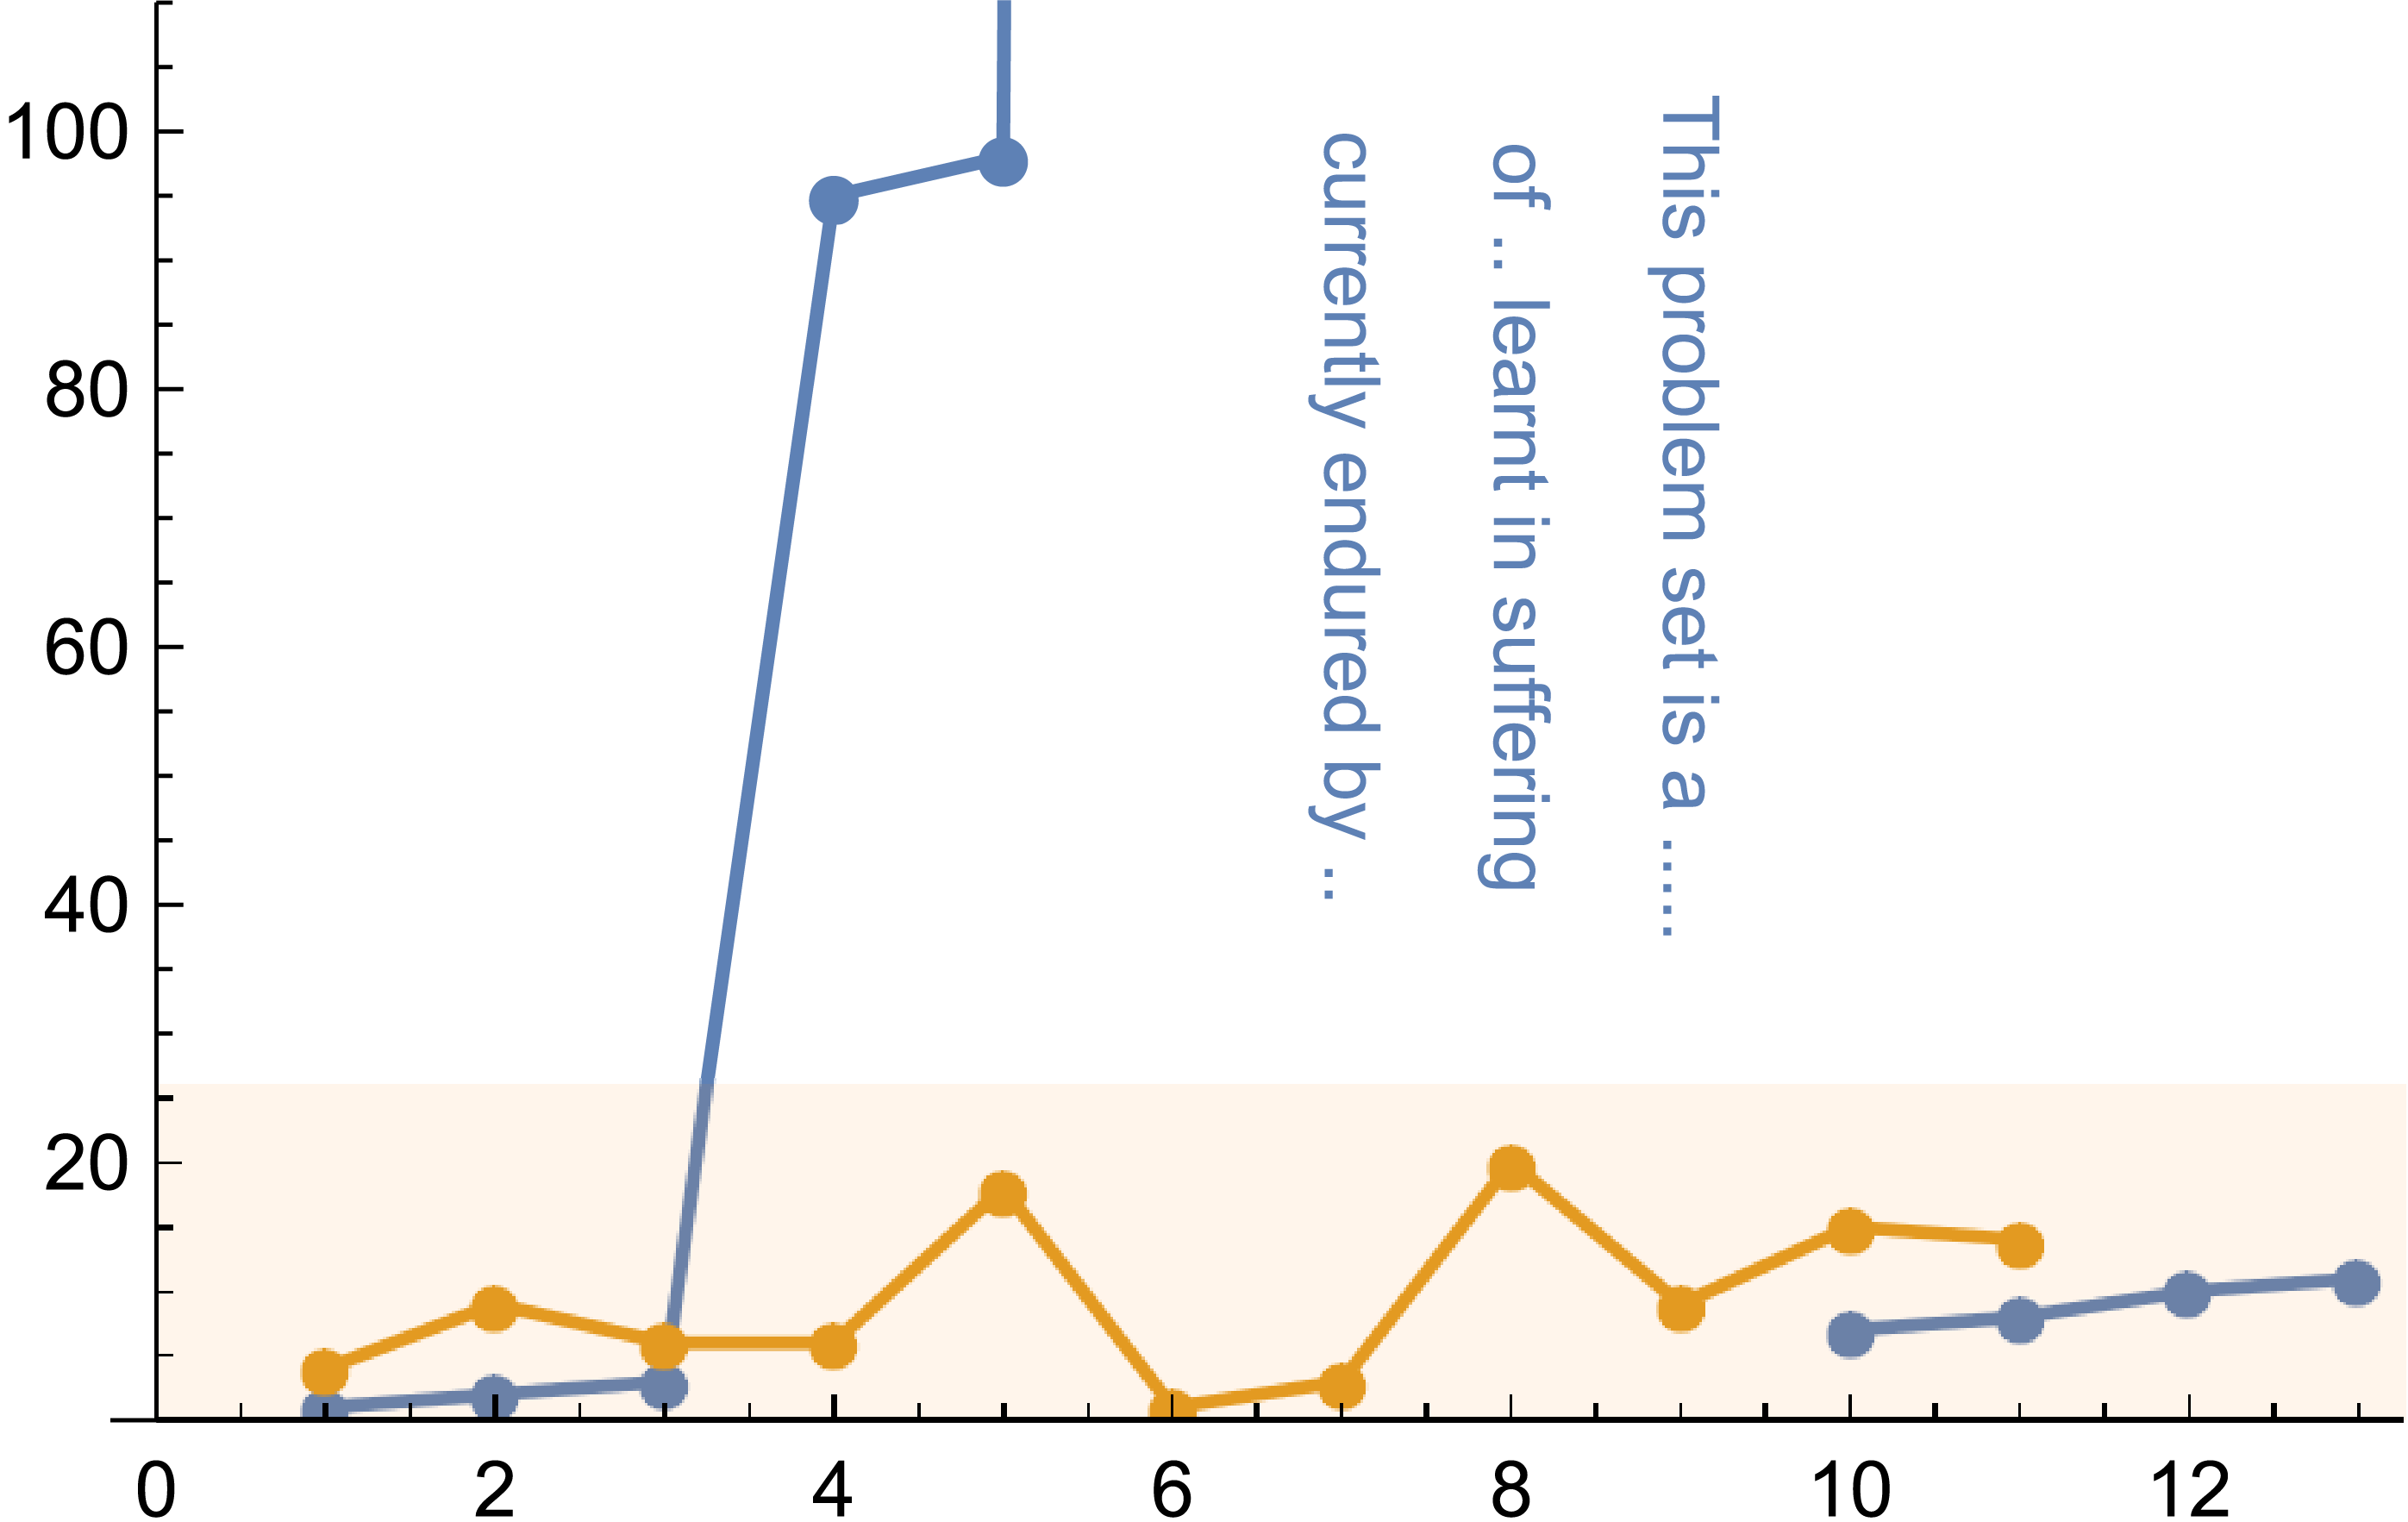
\includegraphics[width=0.72\columnwidth]{0.png}
		
		\small{\textit{(modified from \href{https://ccbc15.cipherpuzzles.com/info/about}{Cipher \& Code Breaking Competition 15})}}
	\end{center}
	\vspace*{\fill}
	
	
	
	
	\setcounter{page}{0}
	
		
	
	
	
	
	
	
	\newpage
	\noindent
	\textbf{前言:这套试题到底是什么?(What Actually is This Problem Set?)}
	
	几个月之前,我得知了某个已经在世界各地使用了十几年的测量方法有严重的问题。并且,尽管只需要高中水平的知识就能对这一偏差做出相当准确的估算,却一直没有人指出它。随后,我将之以一道题目的形式留存了下来,即这套试题中的“题零”——它没有最终出现,但确定了整套试题的基调。此后,我开始收集科研、学业中的各种离谱事情——小到一次不明所以的谈话,大到上百篇忽略了同样的简单事实的论文。这些收集到的内容,加上一些其他的东西,最终统合成了一套试题。
	
	应当很容易注意到,这套试题中包含了一些谜题成分。如果说我对我出的竞赛题有八成的自信,那对谜题大概只有两成的自信。而且,由于没有人帮我测试或验证,这些谜题的质量、难度乃至正确性完全没有保证。建议把它们当作一些彩蛋,或者随便看看剧情,又或者直接跳过。这些谜题的最终结果是一个有意义的英文词组。不过,就算解开了,也完全可以一笑了之——严谨的表述显然不是区区十几个字母能做到的。当然,某些谜题中的某些内容是与竞赛题有关的——有的解释了题目的离谱之处,有的甚至暗示了一部分答案。但既然是谜题,这里就不过多阐释了。
	
	本试题(包括题目和谜题部分)涉及的知识范围参考\href{https://cpho.pku.edu.cn/info/1033/1042.htm}{《全国中学生物理竞赛内容提要》(2015年修订版)}中的决赛内容、\href{https://apho2024.utar.edu.my/Syllabus.php}{亚洲中学生物理竞赛(APhO)大纲}和\href{https://www.ipho2024.ir/page/5}{国际中学生物理竞赛(IPhO)大纲}。我其实并不清楚2024年的一套正常的竞赛题应当是什么题量和难度,所以只是在我认为的竞赛范围内出了一套我认为可以在大约3小时内做完的题目,甚至题目中涉及的很多知识我也只是现学现卖而已。
	
	本试题中与现实世界有对应的信息不代表也不暗示真实情况。特别的,本试题不涉及对特定个人或团体的评价,不应被理解为任何形式的评论、意见或建议。
	
	感谢为我提供出题思路乃至完整题目的HamiltonHuaji大佬和yigo大佬。如果没有他们的帮助,这套题目可能永远也无法完成。
	
	如果你发现了错误或有任何建议,欢迎通过电子邮件 \href{mailto:ridiculoustriplets@gmail.com}{ridiculoustriplets@gmail.com} 与我联系。老年选手算错答案在所难免,还望大家多多包涵。
	
	我想通过这些题目传递一个信息:某些看起来很复杂、很高端、乃至很少有人意识到的问题,实际上有非常简单和清晰的解释。找到这个解释的过程可能并不容易,因为它涉及到发现问题、建立模型、合理近似、估计结果等一系列技能。但说到底,这里面最难的一步其实是,记得使用自己的大脑。仔细想想,拥有一个真正可以工作的大脑其实是一件非常难得、非常幸运的事情,如果弃之不用就太可惜了。
	
	对我而言,出这套题目当然是一个并不算小的时间和精力消耗。但或许更值得在意的是:全世界的科研工作者在这些简单问题上浪费的时间总计肯定大于数万乃至数百万人时。当然,可能也有人从这些有意或无意说错的东西上获得了鲜花、掌声与荣誉——这就是另一个话题了。我无意在这里深入讨论科研圈的体制和评价标准,但在某种意义上,这套题目也算是对此的一些记录吧。
	
	上次出竞赛题已经是$\left(\ket{6}+\ket{7}+\ket{8}\right)/\sqrt{3}$年前的事情了。而这次的尝试与其说是在出竞赛题,不如说是在写一个形式奇特的(不知道多少年的)年度总结,甚至可以说是一种行为艺术。从一开始,夹杂在这些题目中的整活、戏谑与嘲弄可能才是更重要的。出这么一套题对我显然没有什么看得见摸得着的好处,我也不知道它是否会真的对其他人有所帮助。不过,从某种意义上说,这些功利的好处也并没有那么重要。至少在这近两个月的时间里我确实玩得很开心,希望大家也能在这里玩得开心!
	
	\begin{flushright}
		berylliumcopper
		
		二零二四年十一月
	\end{flushright}
	

	
	
	\newpage
	\noindent
	\textbf{小孬剧一:伊丽莎白皇后的最后一封信(The Last Letter Read by Empress Elisabeth)}
	
	\textit{本题满分$0$分。}
	
	\textit{“纵使一圈又一圈的在重复的轨道上加速,终究也追不上光,”茜茜公主念着奇怪的歌谣。\faMapMarker“而在七十二年之后的天空,一颗流星分裂为四,第五块碎片也随后出现。”她拆开了一封信。纸质信的样子就像用于数据处理的公式,很久之前是这样,很久之后也是这样。信的第一行写到:“从来如此的背后,是不言自明而绝不会出错的世间真理,还是愚蠢至极却无自知之明的集体狂欢?”之后是密密麻麻的字母,写了好几页还写不完。}
	
	\textit{她显然是没有时间读完这么多了,直到最终也只是随便看了其中普通的一行,内容是:MOY WVM PCVLZML IVL AQF HCQNA-HHHNN。}\\
	
	\noindent
	\textbf{题一:真的有几十特斯拉的磁场吗?(Is There Really a Magnetic Field of Tens of Tesla?)}
	
	本题满分60分。
	
	在1845年,法拉第首先测量了线偏振光在经过磁场中的介质时的偏振面旋转,即法拉第效应。如图(a)所示,一束角频率为$\omega$的线偏振光正入射长度为$L$、在该频段的折射率为$n(\omega)$的透明介质。介质表面法向为直角坐标系$z$方向,外加磁场$B$也沿$z$方向。此时,从介质中出射的光线的偏振面相对于入射光线旋转了角度$\theta$。该效应可以用右旋圆偏振光和左旋圆偏振光
	的折射率之间存在一个微小的差异来解释。(本题中的右旋圆偏振光定义为当从源点顺着传播方向看去时,空间中一固定位置的平面上的电场强度随时间顺时针旋转。)本题将基于经典电磁学理论,讨论一个法拉第效应的模型,并将此模型推广到与法拉第效应相关的其他效应上。不考虑相对论电磁学和量子效应\footnote{应当指出,在严格处理该问题时,可能需要涉及量子力学和微扰理论。题目中的经典模型只能给出一个阶数正确的粗略估算。},不考虑带电粒子加速运动所产生的电磁辐射及其带来的能量损耗。
	
	为简化起见,假设介质中只有两种带电粒子,分别为正带电粒子(电量$+e$)和负带电粒子(电量$-e$)。两种粒子的质量分别为$m_i$和$m_e$,粒子数密度均为$N_c$。考虑粒子在$xy$平面内的运动。已知当两种粒子偏离平衡位置的位移分别为$\vec R=(R_x,R_y)$和$\vec\rho=(\rho_x,\rho_y)$时,单位体积内的势能为
	\begin{equation*}
		V(\vec R,\vec\rho)=N_c\left[\frac{m_i\Omega_i^2}{2}(R_x^2+R_y^2)+\frac{m_e\Omega_e^2}{2}(\rho_x^2+\rho_y^2)+\delta\vec{R}\cdot\vec{\rho}\right]
	\end{equation*}
	其中$\delta,\Omega_i,\Omega_e$为已知常数。已知该介质中的光速可以表述为$c/n(\omega)=1/\sqrt{\varepsilon\mu_0}$,其中$\varepsilon$为介电常数。真空介电常数$\varepsilon_0$、真空磁导率$\mu_0$和真空光速$c=1/\sqrt{\varepsilon_{0}\mu_0}$为已知量。忽略带电粒子运动时的受到的任何阻力和耗散。
	
	(1)试计算在图(a)所示的情形下,右旋圆偏振光和左旋圆偏振光的介电常数的差异$\Delta\varepsilon=\varepsilon_R-\varepsilon_L(|\Delta\varepsilon|\ll\varepsilon_{0})$和折射率的差异$\Delta n=n_R-n_L(|\Delta n|\ll1)$。进而证明在法拉第效应中,光线偏振面的旋转角度满足
	\begin{equation*}
		\theta=S(\omega)LB
	\end{equation*}
	其中$S(\omega)$称为韦尔代常数。给出$S(\omega)$的表达式。假设入射光的光强足够低。
	
	如图(b)所示,一束角频率为$\omega$的右旋圆偏振光正入射长度为$L$的透明介质,外加磁场为零。此时,介质中将出现一个非常小的磁化,即逆法拉第效应。在经典模型中,这一效应可以由带电粒子在周期性光场的驱使下的运动来解释。
	
	(2)试证明,介质中由于入射光场而产生的沿$z$方向的磁化强度(单位体积内的磁偶极矩)可以表示为
	\begin{equation*}
		M=T(\omega)E_0^2
	\end{equation*}
	其中$E_0$为光场在介质中的振幅(电场强度)。据此给出$T(\omega)$与$S(\omega)$之间的关系(用普适常数和$n(\omega)$、$\omega$、$e$表示)。
	
	为了测量逆法拉第效应产生的磁场,有人设计了如图(c)所示的实验。一束角频率为$\omega_0$、电场强度为$E_0$的右旋圆偏振光正入射长度为$L$的透明介质。同时,一束角频率为$\omega_1$、电场强度振幅远小于$E_0$的线偏振光也从相同方向正入射该介质。两束光在空间上实际是重合的,图中为清楚起见将它们分开了。实验上观察到了线偏振光$\omega_1$的偏振面在通过介质后的旋转。
	
	取:$\Omega_i=2\pi\times1.00\times10^{13}\,\text{Hz}$、$\Omega_e=2\pi\times2.40\times10^{14}\,\text{Hz}$、$\omega_0=2\pi\times1.20\times10^{13}\,\text{Hz}$、$\omega_1=2\pi\times6.00\times10^{14}\,\text{Hz}$、$n(\omega_0)=2.0$、$n(\omega_1)=1.7$、$L=100.0\,\mu\text{m}$、$e=1.6\times10^{-19}\,\text{C}$、$m_i=4.2\times10^{-26}\,\text{kg}$、$m_e=9.1\times10^{-31}\,\text{kg}$、$N_c=2.0\times10^{27}\,\text{m}^{-3}$、$\delta=0.100\,\text{N/m}$、$E_0=4.0\times10^8\,\text{V/m}$、$\varepsilon_{0}=8.85\times10^{-12}\,\text{F/m}$、$\mu_0=4\pi\times10^{-7}\,\text{H/m}$、$c=3.00\times10^8\,\text{m/s}$。
	
	(3)试分别计算此时正带电粒子和负带电粒子做圆周运动的半径大小。在上述几何位形下,若外加磁场为零,则介质中的磁感应强度大小约为$B\sim\mu_0M$,其中$\vec M$为介质中的磁化强度。若取$\vec B=\mu_0\vec M$,并假设该磁场通过法拉第效应使得线偏振光$\omega_1$的偏振面旋转,试求预期的旋转角$\theta_F$。本问中的数值结果保留两位有效数字。
	
	将实验中测到的偏振旋转角度$\theta_E$代入法拉第效应的表达式$\theta_E=S(\omega_1)LB$,可以推算出磁感应强度约为数十特斯拉。基于此,有些人认为他们在介质中实际产生了对应大小的磁场。然而,该结果与你在(3)中计算出来的结果有很大差异。对于这一差异,一种理解是:此处通过偏振旋转角度反解出的磁场并非介质中实际存在的磁场,而只是对介质中带电粒子运动产生的效应的一种等价描述。
	
	(4)等效磁场的主要来源是正负带电粒子相互作用项对能量的二阶微扰,与光学中的二阶非线性效应是同阶修正。为估算该修正的大小,对负带电粒子坐标$\vec\rho$,引入一个很小的非中心对称势场
	\begin{equation*}
		\Delta V(\vec\rho)=\kappa\rho_x^3
	\end{equation*}
	其中$\kappa=2.0\times10^9\,\text{N/m}^2$。基于该模型,以下一系列问题提示了一个用于估计等效磁场的数量级的方法。这里的所有估算结果都应给出具体数值,但只要求数量级正确,不要求正负号和矢量的方向。估算所采用的方法应当是物理上合理的。
	
	(4.1)此时,负带电粒子的运动轨迹将不再是正圆,轨迹中心相对坐标原点将会有一个微小的偏移$\rho_{\kappa}$。试估计$\rho_{\kappa}$的大小。
	
	(4.2)通过正负带电粒子之间的相互作用势$\delta\vec R\cdot\vec\rho$,负带电粒子运动轨迹的偏移将导致正带电粒子的运动轨迹中心也出现偏移$R_{\kappa}$。试估计$R_{\kappa}$的大小。
	
	(4.3)上述偏移会导致每个正带电粒子在势场中的能量出现微小变化。另一方面,运动的正带电粒子可以视为小电流环,能量的微小变化也可以由其在假想外磁场$B_{eff}$中的磁能来解释。认为两种解释给出的能量变化相等,试据此估计等效磁场的磁感应强度$B_{eff}$。
	
	\begin{figure}[!bh]
		\centering
		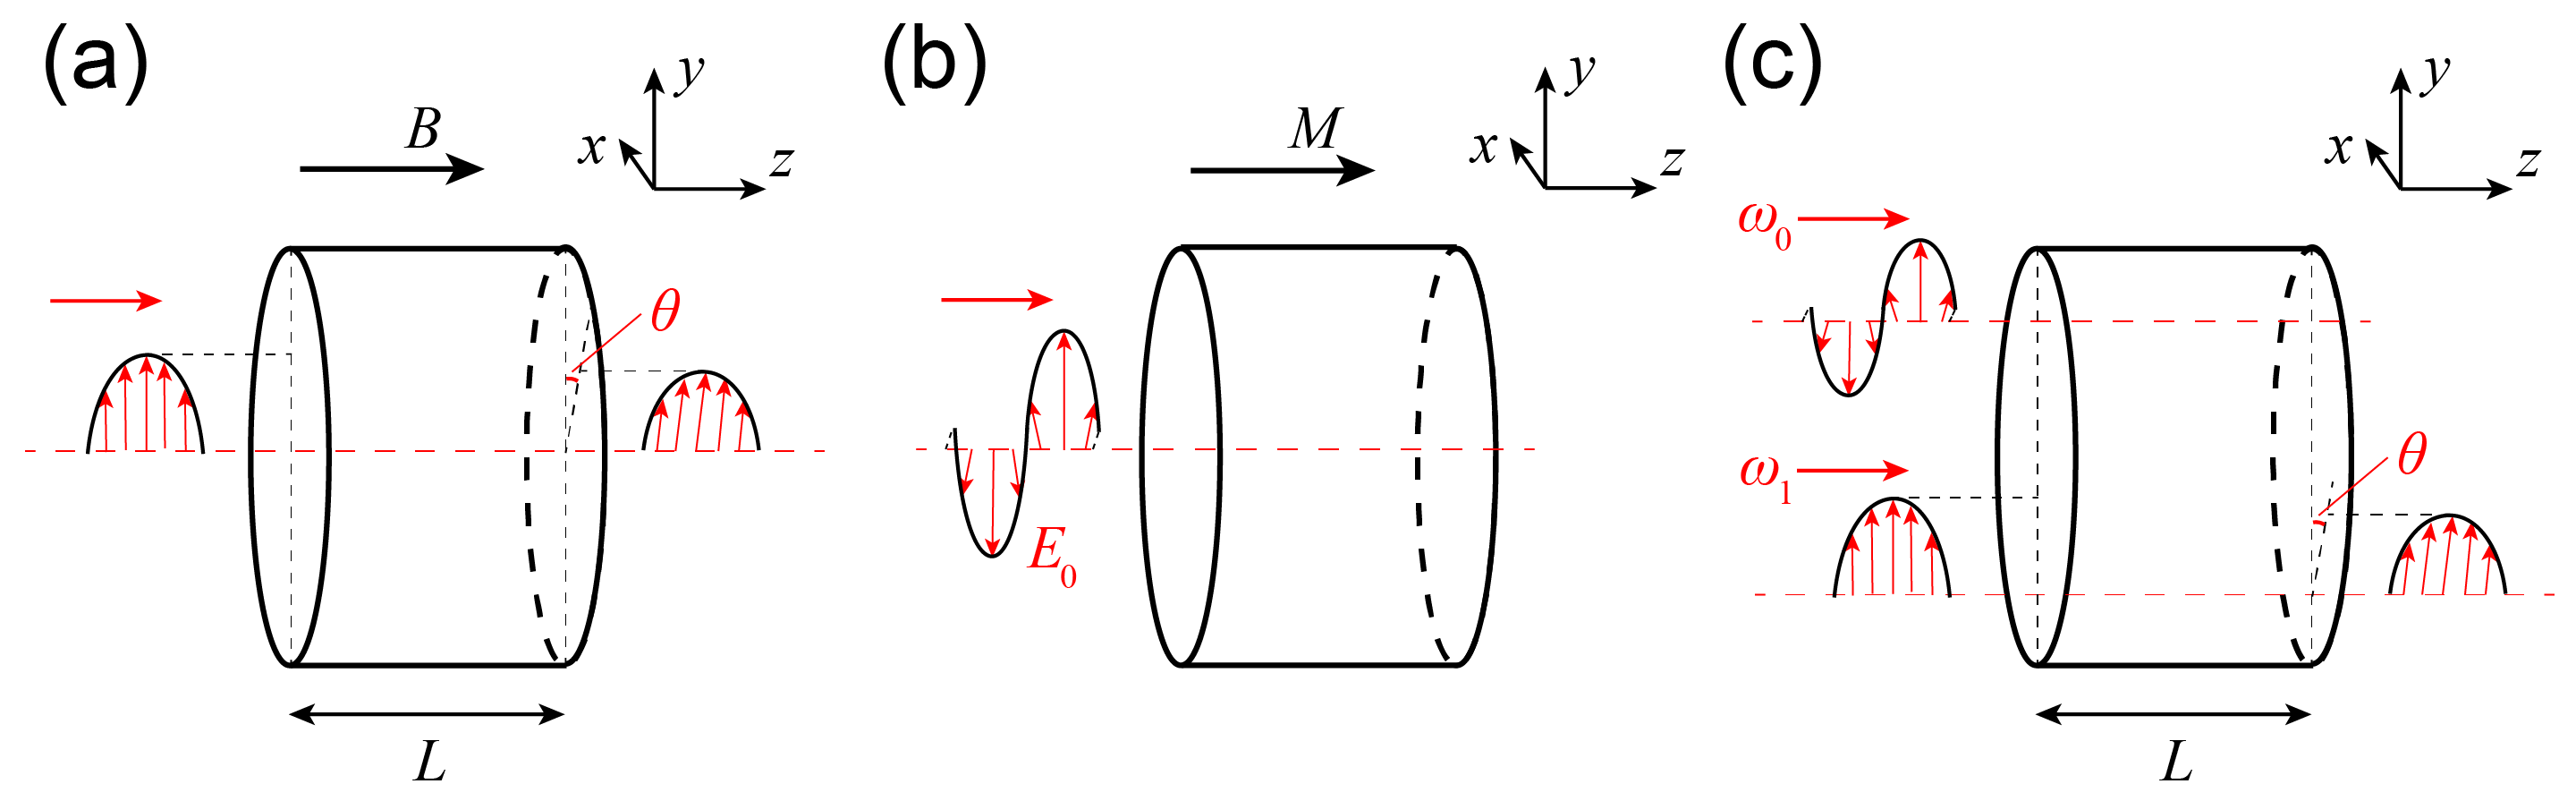
\includegraphics[width=0.99\columnwidth]{2.png}
	\end{figure}
	
	\newpage
	\noindent
	\textbf{小孬剧二:不尽真实的凝聚态与皆为虚假的守恒律(Not-So-Real Condensed Matter and Truly-So-Fake Conservation Law)}
	
	\textit{本题满分$0$分。}
	
	\textit{00432510:凡凝聚态间至真之理,莫过于二二之方阵。倘有多者,或未尽简,或实谬哉。}
	
	\textit{00410542:(仅作为示例)($-$1/$-$8)}
	$$p(x)\ud x=A\left(\frac{6}{(1+\ue^{(20-x)/3})(1+\ue^{(x-55)/4.91})}+3\ue^{-(x-96)^2/71}\right)\ud x, x\in[0,100]$$
	
	\textit{(三年零十分钟后)}
	
	\textit{甲:动量守恒啊、能量守恒啊,肯定是好的。但是呢,在应用这些东西的时候,要遵循对应的条件。在空气和样品的界面处,光在空气中入射的波矢$k$和样品中出射的波矢$k$可以不一样。你们不要老想着搞个大新闻,说我这里违反动量守恒定律了。}
	
	\textit{(又二十分钟后)}
	
	\textit{乙:我还是不能理解为什么入射的k和出射的k不一样,动量守恒都不要了吗?}
	
	\textit{(又一年后)}
	
	\textit{%23/24-2-00432150-1:
	“这……你是做凝聚态的是吧……那么这……你做的这……材料的这……空间群是什么?不准查这……晶体结构的网站……等等,是什么网站来着?这……刚梦见从欧洲回来这……还在倒时差呢……”\faMapMarker}\\
	
	
	
	\noindent
	\textbf{题二:动量是否守恒?(Is Momentum Conserved?)}
	
	本题满分60分。
	
	离子晶体中的电子云的偏移和离子实的运动所对应的时间尺度有着明显的不同。这是因为电子和离子实的带电量(的绝对值)相当,因而相互作用的强度相近,但电子的质量仅为离子实质量的$<10^{-3}$量级。然而,电子云和离子实都可以与电磁场发生相互作用,这也就意味着在处理此类问题时经常需要将这两部分的贡献分开计算。本题就是要讨论这种方法。
	
	下面分别简要说明如何处理电子云的电偶极矩和离子实的电偶极矩。电子云的响应速度很快,在本题所涉及的时间尺度下可以认为是瞬时的,其对应的电极化强度$\vec P_e$与电场强度$\vec E$的关系为
	\begin{equation*}
		\vec{P}_e(t)=\chi\vec E(t)
	\end{equation*}
	其中$\chi$为已知常数。而离子实的电偶极矩与具体的晶体结构和离子实偏离平衡位置的位移有关,可以等效为将每个离子实都视为带对应电量的点电荷时的电偶极矩,并由此得到离子实的电极化强度$\vec P_m$。晶体整体的电极化强度为电子云和离子实两部分之和,即
	\begin{equation*}
		\vec P=\vec P_e+\vec P_m
	\end{equation*}
	
	考虑一个如图(a)所示的离子晶体晶格,由带正电量$+Q$的A离子和带负电量$-Q$的B离子组成。图(a)中红线由一系列边长为$a$的正方体相接地拼成。在平衡位置,所有离子都在这些正方体的顶点上,两种离子各自构成一晶格常数为$2a$的面心立方晶格。此时晶体中的(宏观)电极化强度$\vec P=0$。
	
	下面我们考虑离子略微偏离平衡位置的情况。假设将所有的A离子相对B离子均向同一方向移动距离$d\ll a$,则在晶体内的宏观电场始终为零的情况下,单位体积内晶体的能量的增加值可以表示为
	\begin{equation*}
		V_p(d)=\zeta d^2
	\end{equation*}
	其中$\zeta$为已知常数。已知每个A离子的质量为$m_A$,每个B离子的质量为$m_B$。不考虑任何阻尼或耗散。真空介电常数$\varepsilon_{0}$、真空磁导率$\mu_0$、真空中光速$c=1/\sqrt{\varepsilon_{0}\mu_0}$视为已知量。
	
	(1)显然,在该模型下,晶体的介电常数(或绝对电容率)$\varepsilon$不再是一个与外加电场的角频率$\omega$无关的常量。试计算该晶体在$\omega=0$时的静态介电常数$\varepsilon_{st}$,以及在$\omega$很大(但仍远小于电子云的特征响应频率,一般对应可见光区)时的高频介电常数$\varepsilon_{\infty}$。
	
	考虑晶体中沿某一晶轴方向$+z$传播的平面波元激发,其角频率为$\omega$、波矢为$k=2\pi/\lambda\ll 1/a$(所以,这些物理量发生显著变化的空间尺度远大于晶胞尺度)。不失一般性,我们可以将此时晶体中A离子的位移$\vec{r}_A$、B离子的位移$\vec{r}_B$、电场$\vec E$表述为(振幅$\vec R_A,\vec R_B,\vec E_0$也为复数,整个式子的实部表示物理上可观测的值)
	\begin{equation*}
		\vec r_A(x,y,z,t)=\vec R_A\ue^{\ui(kz-\omega t)}
	\end{equation*}
	\begin{equation*}
		\vec r_B(x,y,z,t)=\vec R_B\ue^{\ui(kz-\omega t)}
	\end{equation*}
	\begin{equation*}
		\vec E(x,y,z,t)=\vec E_0\ue^{\ui(kz-\omega t)}
	\end{equation*}
	
	(2)我们关心的是晶体中任意部分不出现宏观运动的情况。亦即:任取一宏观足够小、微观足够大的体积元,其中所有离子实的质心不发生运动。
	
	(2.1)由此给出$\vec R_A$和$\vec R_B$之间满足的关系。
	
	(2.2)若$\vec R_A,\vec R_B,\vec E_0$均平行于$z$轴,电磁学理论给出电位移矢量$\vec D=0$(电磁波是横波)。试求此时的振动频率(即纵光学声子频率)$\nu_{LO}=\omega_{LO}/(2\pi)$。
	
	(2.3)若$\vec R_A,\vec R_B,\vec E_0$均垂直于$z$轴,求解电磁波传播理论(麦克斯韦方程组),得到
	\begin{equation*}
		k^2\vec{E}(x,y,z,t)=\omega^2\mu_0\vec{D}(x,y,z,t)
	\end{equation*}
	据此求解色散关系$\omega(k)$。你应当得到两个分支。讨论当$k$很大(但仍远小于$1/a$)时,两个色散关系的渐近行为。其中一个分支的频率趋于有限值,试给出该值(即横光学声子频率)$\nu_{TO}=\omega_{TO}/(2\pi)$。
	
	(2.4)取NaCl的真实数据:$2a=564\,\text{pm},\varepsilon_{st}=5.9\varepsilon_{0},\varepsilon_{\infty}=2.25\varepsilon_{0},\nu_{TO}=4.9\times10^{12}\,\text{Hz}$,试求$\nu_{LO}$。进而将你在(2.2)和(2.3)中得到的所有三个色散关系$\omega(k)$定性正确的画在同一张图上,横坐标为波矢$k$,纵坐标为角频率$\omega$。
	
	上面(2.2)问中算出的元激发称为纵光学声子,而(2.3)问中算出的元激发称为极化子。极化子的实质是电磁波(光子)与晶格振动(声子)的混合。与光子相似,其能量也是量子化的,一个极化子携带能量$\hbar\omega$和动量$\hbar k$。在固体物理中,量子化条件给出的动量$k$是等间距分布的,因此对于极化子的每个分支,在$k$至$k+\ud k$之间存在的极化子态的数目$\ud N$正比于$\ud k$。
	
	极化子可以由对应频率的光子产生。如图(b)所示,角频率为$\omega_l$、波矢为$k_l=\omega_l/c$的光束从真空正入射一块表面法向为晶格$z$方向的样品,其中的极化子(在$0<k\ll1/a$的范围内)可以用你在(2)中得到的色散关系描述。这样的一个光子在样品表面只产生一个角频率为$\omega$、波矢为$k$的极化子。
	
	(3)试判断上述过程中$\omega$是否必须等于$\omega_l$?$k$是否必须等于$k_l$?说明理由。假设一束光激发极化子的效率正比于能够满足以上条件的极化子态数目,那么应当如何选取其角频率$\omega_l$才能使激发效率最高?用$\omega_{LO}$和$\omega_{TO}$表示你的结果。
	
	\begin{figure}[!bh]
		\centering
		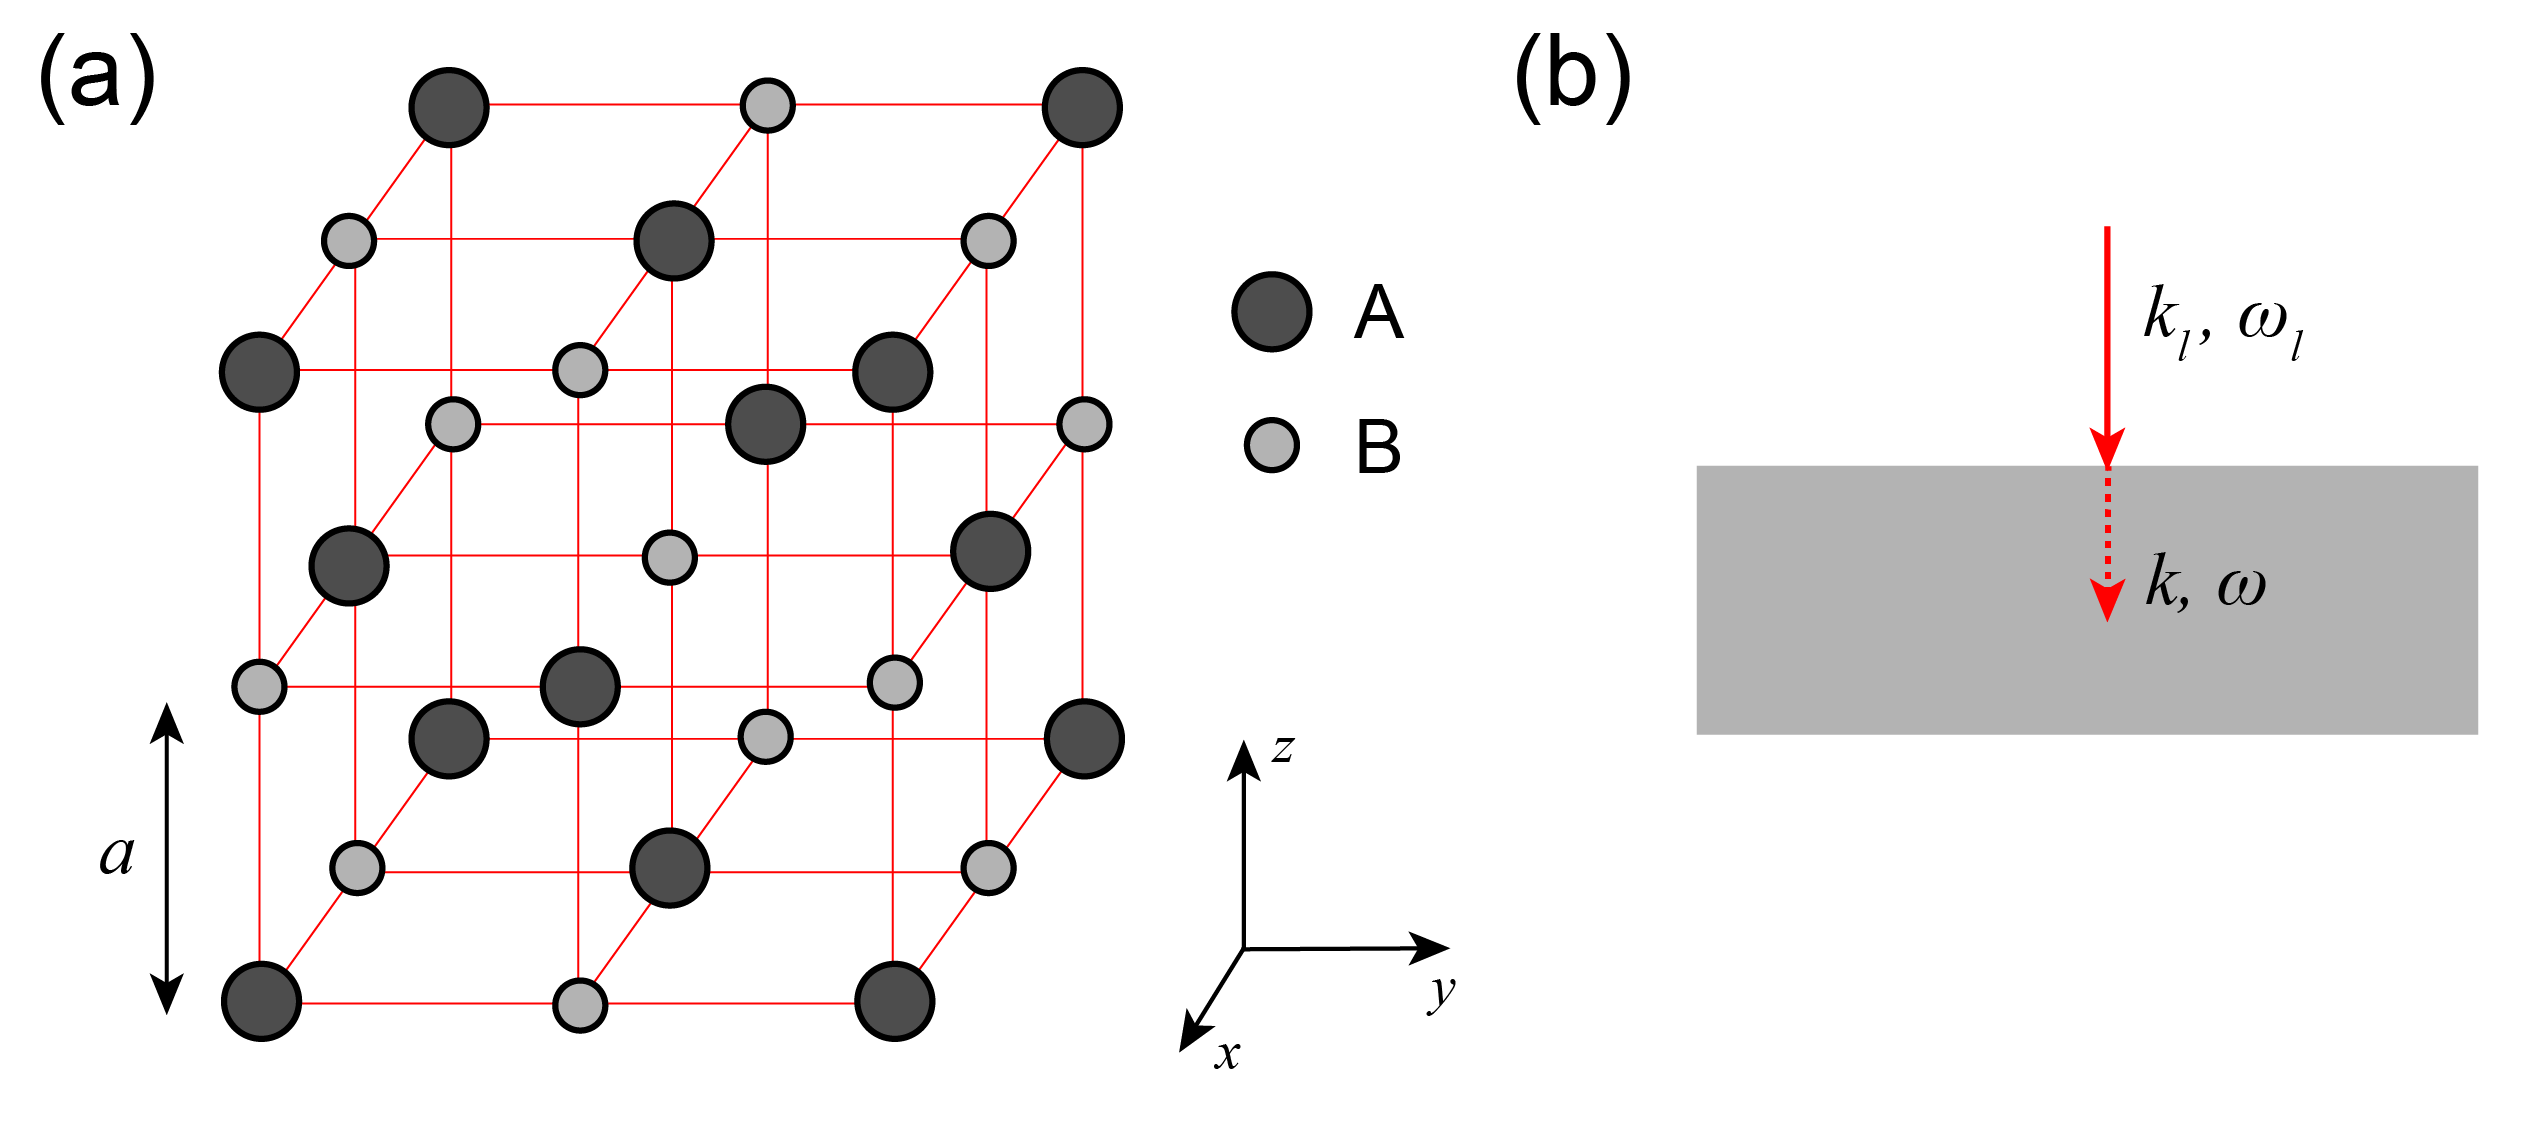
\includegraphics[width=0.9\columnwidth]{3.png}
	\end{figure}
	
	
	\newpage
	\noindent
	\textbf{小孬剧三:音乐剧、图灵与人工智能(Musical, Turing, and Artificial Intelligence)}
	
	\textit{本题满分$20\ui$分。}
	
	\textit{说明:除“题三”外的所有部分中,只有“小孬剧三”中含有与“题三”的分数相关的提示。}
	
	\textit{“路易吉·卢切尼,别再胡说八道什么图灵和人工智能了!音乐剧到底在哪里?这背后有什么阴谋?”}
	
	\textit{“哇啊啊啊啦啊啊!音乐剧明明到处都是啊!看看这些尊贵的曲目的名字吧,下面的话里处处都能证明这一点……”}
	
	\textit{(12,2,8)}
	
	\textit{甲:现在人们都说,掌握人工智能和机器学习要从娃娃抓起。}
	
	\textit{乙:你这孩子还真的是孩子吗?这是小小年纪就背负了世界的重担啊……}
	
	\textit{甲:架不住人家机器学习就是有用啊!}
	
	\textit{乙:要是我家小孩小时候学这个,我会觉得是看了什么不该看的东西。虽然表情上故作正经,心里却比见了狼还慌张。——啊不对,我连女朋友都找不到,哪来的孩子啊?}
	
	\textit{甲:你看,人工智能就能解决这个问题。给你安排一个AI天才猫娘女友,然后你们俩原地结婚,不就行了?}
	
	\textit{乙:别,你这让我感觉婚礼上回答问题说“我愿意”的时候背后会有一群跳着僵尸舞唱着怪歌词的家伙跟着起哄……}
	
	\textit{(15,3,7,13)}
	
	\textit{甲:最近大家都在提这几条改进建议,你却跟没看见一样。}
	
	\textit{乙:总不能人家说啥我就听啥吧?我最近还真没看到过什么有价值的建议。说不定就是几个人闲得无聊喝咖啡的时候一合计,开玩笑的说什么末日要来了,就弄出来好些一模一样的建议。这有什么代表性吗?}
	
	\textit{甲:你动动手指就行了,把这条消息一删,万事大吉。}
	
	\textit{乙:可不是你说的那么轻巧啊。删是删的容易,可恢复起来就困难了。到时候你可别坐在坟头上哭着问人家在哪,哪怕想隧穿到连续剧的下一集都来不及了。}
	
	\textit{甲:你还是来自己看看是怎么回事吧:}
	
	\textit{This message in the archive is too ridiculous and should be deleted:}
	
	\textit{Texnikaly, de Speling of English in dis Sentens is modifid to mak it mor tradisnal, mor vizibl, mor unik to Pronunsiasn, and mor kompatibl wid Tex. (89/01/30)}
	
	\textit{乙:我倒觉得这条记录很有意思。咱们得先是个archive,再看怎么变成别的……这就像是在夜里开船,一定要注意自己的方向,别把真正的目的忘记了……}
	
	\textit{(3,5,2)}
	
	\textit{甲:如果图灵能看到今天的人工智能研究的论文,那该有多高兴啊!}
	
	\textit{乙:如果他看到今天计算机的算力应该确实会很高兴……但如果说论文嘛,那就得要看具体是那一篇文章了。有时候呢,算法本身是好的,可是用它的人呢就跟旅游景点里面卖劣质纪念品的小贩一样。人家景点再厉害也跟你手里的破玩意没有半点关系。}
	
	\textit{甲:我没听明白。}
	
	\textit{乙:QVBYUHS KL SLJVSL WVSFALJOUPXBL DRSBDOOX IIRDBOOO。}
	
	\textit{甲:这就更看不懂了。}
	
	\textit{乙:再打个比方,求由波函数$\Psi(r,\theta,\phi)\propto(r^4+395391r^2+116587329612)\ue^{-r/454}$所描述的粒子离原点的距离$r$的期望值(3/$-$5)。}
	
	\textit{甲:我算出来了,是$1810.04703$!}
	
	\textit{乙:一看你就是漏乘了个东西。罢了,用你能听懂的话再说一遍吧——要是老爹自己不怎么正经,那生出来的也一样不正经。}
	
	\textit{甲:我甚至都分不清楚你这个“不正经”是褒义还是贬义。}
	
	\textit{乙:倒也不需要弄清楚。我只是在想,如果大家都觉得连基本的物理定律都不需要管了,只要随便把数据丢进机器学习的代码里,带上ML的标签能发论文就行,那又何尝不是在将要沉没的破船上表演最后的疯狂呢……死神什么时候这么近了?}\\
	
	\noindent
	\textbf{题三:研究物理不如研究机器学习(It is Better to Study Machine Learning Than Study Physics)}
	
	本题满分$50+20\ui$分。
	
	动作捕捉技术在游戏、影视等领域有着重要的应用。记录下演员的真实动作之后,动画师在计算机中的动作建模就有了基础。动作捕捉的一种方案是记录演员身上的特征点出现在摄像机中的位置,再将多个摄像机中的信息组合起来。这种方案准确度很高,但不能在狭小空间中使用,且摄像头阵列的成本非常高。另一种方案是在动捕演员身体的合适位置上安装加速度计,通过加速度反解出身体上各位置的位移,进而给出动作位形。理论上,只要演员的初始动作已知,通过数值积分即可获知之后的运动情况。但在实际的应用中,这一方案中的噪声和误差会随时间累积,导致准确性较低。在2024年之前,人们一直在尝试利用机器学习将加速度计的读数与演员动作进行对应,却没有注意到对体系的建模中存在系统误差。本题将定量研究该系统误差,进而讨论它是如何使反解的位置信息显著偏离演员的实际动作的。本题中的数值结果均应写成保留三位有效数字的形式。
	
	忽略演员腿部的运动,建立如图(a)所示的简化模型。身体主体被模型化为宽为$b$,高为$H$的薄板,其左右两侧高度为$h$处分别由关节A和A$'$(肩关节)连接长为$c$、质量为$2m$的匀质细杆,代表两条大臂。两条大臂顶部由关节B和B$'$(肘关节)分别连接长也为$c$、质量为$m$的匀质细杆,代表两条小臂。建立地面参考系$S_0(x_0,y_0,z_0)$(认为是惯性系)和随身体主体一起运动的参考系$S_1(x_1,y_1,z_1)$。两坐标系在$t=0$时重合,此时坐标原点均在身体主体薄板的几何中心,$x$方向沿身体薄板方向,$z$方向竖直向上。在身体中心O和小臂顶端C和C$'$各安装一个加速度计和一个角速度计,从而可以测量坐标系$S_1$相对$S_0$的运动,以及C点(在惯性参考系中)的加速度$\vec a_0(t)$。
	
	在2024年之前,该领域中通用的算法是:计算$\vec a_0(t)$在$S_1$坐标轴上的投影$\vec a_0(t)=a_{0,x1}\hat x_1+a_{0,y1}\hat y_1+a_{0,z1}\hat z_1$。认为这就是C点在$S_1$参考系中的加速度,对时间两次积分得到C点在$S_1$参考系中的运动轨迹。
	
	(1)试阐释该算法错在哪里,并直接写出一个公式说明其与正确算法之间的差异。
	
	设在$t=0$时刻,水平地面上的动捕演员的两大臂竖直向上,两小臂顶端C和C$'$交于身体中心正上方,如图(b)所示。然后,其身体开始绕过身体中心的竖直轴线以角速度$\Omega_0$逆时针旋转,同时两臂对称的逐渐张开。在$0<t\leq\tau=1/\Omega_1$的时间范围内,两臂张开的运动可模型化为肘关节不动,而肩关节以$\Omega_1$的角速度匀速转动。运动过程中,身体主体始终垂直于地面,两截手臂与身体主体始终在同一平面内。图(c)画出了某一时刻$t\in\left(0,\tau\right]$的演员身体的位形,其中标出了各转动角度。
	
	给定以下数据:$\Omega_0=1.100\,\text{rad/s}$、$\Omega_1=0.800\,\text{rad/s}$、$b=40.0\,\text{cm}$、$H=175.0\,\text{cm}$、$h=150.0\,\text{cm}$、$c=32.0\,\text{cm}$、$m=2.10\,\text{kg}$。重力加速度取为$g=9.80\,\text{m/s}^2$。
	
	(2)若采用上述错误的算法,试计算积分之后得到的$t=\tau$时刻C点在$S_1$参考系中的位置$\vec r_{1}^\star(\tau)$,及其与正确的位置$\vec r_1(\tau)$之间的距离。注意到在$t=0_+$时刻,C点在$S_0$和$S_1$参考系当中的位置和速度矢量均相同,可以此作为积分的起点。
	
	(3)肩关节A处的连接所产生的效果可等价为过A点的作用力加上以A点为转轴的力矩。试计算在$t=\tau/2$时刻,肩关节A对大臂的力矩沿$z_1$方向的分量。
	
	\begin{figure}[!bh]
		\centering
		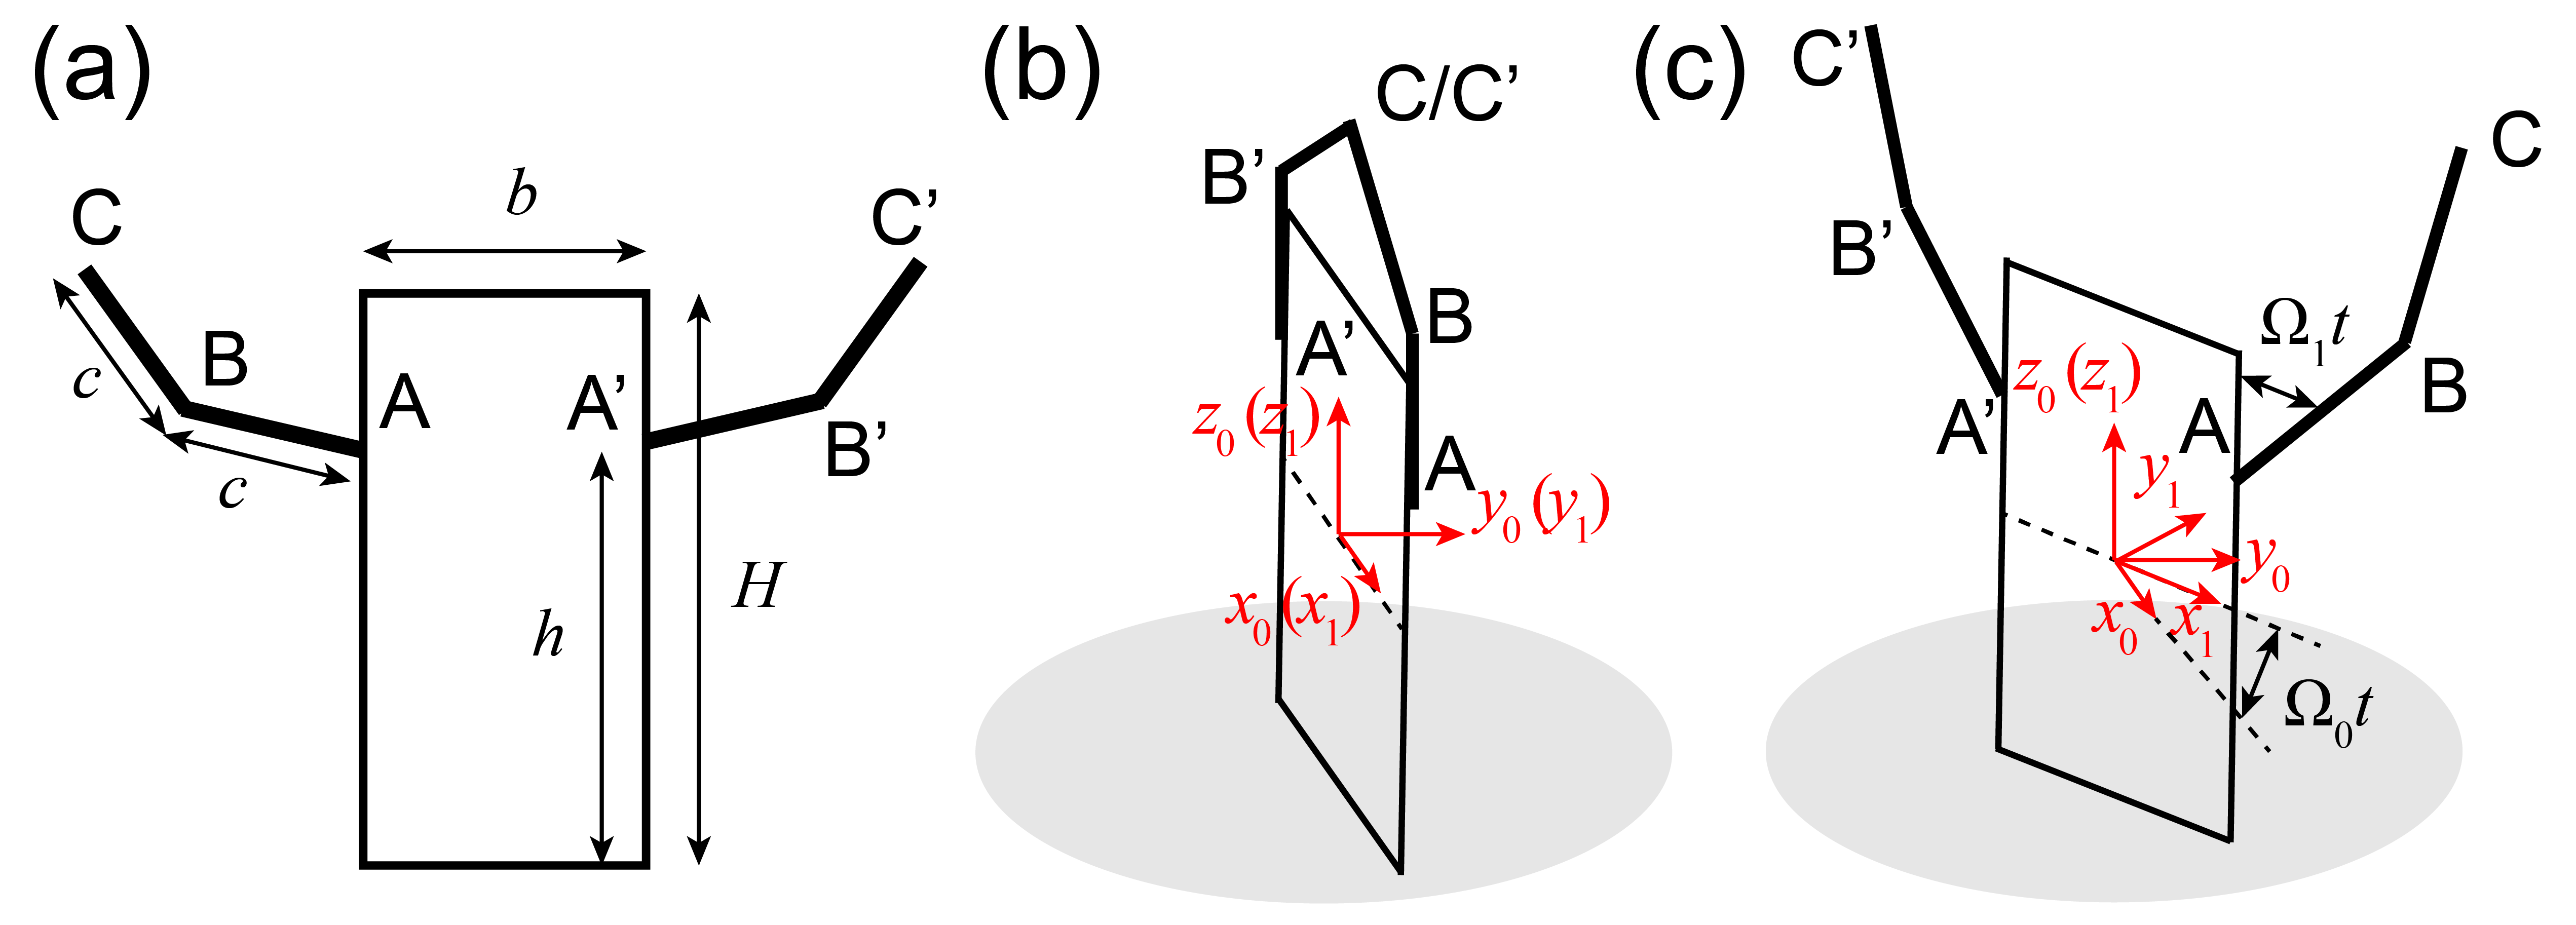
\includegraphics[width=0.96\columnwidth]{4.png}
	\end{figure}
	
	
	
	
	
	
	
	
	
	
	
	
	
	
	
	
	
	
	
	\newpage
	\noindent
	\textbf{小孬剧四:老师好,老师坏(Some Teachers are Good, Others are Bad)}
	
	\textit{本题满分$0$分。}
	
	\textit{虽然分数不是万能的,但是分数给的太差是万万不能的。}
	
	\textit{“听说在这里,百分制下85分及以上的人数占比能达到40\%就已经是极好甚至最好的给分了。这是怎么回事呢?”}

	\textit{1. 一位少年班同学2019年4月3日的日记}
	
	\textit{今天是我十七岁的生日,同学们祝我生日快乐的时候都说我是为绩点而生的。我觉得这句话怎么听怎么别扭,但又不知道是什么意思,也不知道怎么反驳。其实我绩点并不高,今天看到k\=eng课出的分,更是差点晕过去。听说这课的最高绩点4.3只有一个人,4.0的人占20\%,3.7的人占30\%,3.3的人占40\%,3.0的人占5\%,结果给了我一个2.3。气死我了!说来也是奇怪,别的课都是学期末出分,也就这一门课是4月3日出分了。本来今天就心情郁闷,结果晚上开了一小会游戏就提示我本周的未成年人游戏时间限制到了,不让我接着打了。唉,怎么有大学生打不了游戏啊!真是受不了了!}
	
	\textit{2. 01233170:“投资学导论”(4/0)}
	$$p(x)\ud x=\left[\frac{25317}{A}\delta(x-85_-)+\frac{16878}{A}\delta(x-100_-)\right]\ud x, x\in\left[0,100\right]$$
	
	\textit{3. 00432108:“只是求导和积分而已”(0/$-$7)}
	$$p(x)\ud x=\frac{1}{30}\left[0.4\ue^{(x-98)/10}+\frac{A}{1+\ue^{(x-62.95)^2/136.86}}\right]\ud x, x\in[0,100]$$
	
	\textit{4. 00432150:“考试内容是解薛定谔方程”($-$2/$-$5,$-$1/$-$2,1/0)}
	$$p(x)\ud x=A_1\left[\ue^{-(x-65)^2/721}+0.4\ue^{-x/9}\right]\ud x, x\in[0,100]$$
	$$p(y)\ud y=A_2\left[5\delta(y)+A_3\frac{\ue^{-(u-65)^2/721}+0.4\ue^{-u/9}}{\sqrt{30(4-y)}}\right]\ud y, y\in(0_-,0_+)\cup[1,4]$$
	\textit{其中$u(y)=100-\sqrt{1600(4-y)/3}$。}
	
	\textit{5. 一个德国的石头(当然,也可以是奥地利的)}
	
	\begin{table*}[!h]
		\centering
		\begin{tabular}{|c|ccccc|}
			\hline
			\textit{成绩}&1&2&3&4&5 \\
			\hline
			\textit{人数}&21&8&1&0&0 \\
			\hline
		\end{tabular}
	\end{table*}
	
	
	\textit{6.在考试开始之前……}
	
	\textit{\fbox{竞赛教员}:你们上午的考试延长时间了吗?如果延长了,我们是否要将下午的考试也一并推迟一下?放心,我下午的考试很友好,你们不用担心分数,也不会影响你们吃晚饭的。}
	
	\textit{同学:我们上午没有延长。}
	
	\textit{\fbox{竞赛教员}:上午的考试……统计物理的那一半是很好的,但另外一半出成那个样子,你们也没有延长?}
	
	\textit{同学:老师,那些题目再怎么延长我们也还是不会做。这个老师上课讲的东西我们都听不懂,下课去问也不回答。}
	
	\textit{\fbox{竞赛教员}:啊……你们好好考下午的考试吧。考完之后还有更重要的事情需要由你们来完成……}\\
	
	\noindent
	\textbf{题四:多次反射如何相加?(How to Add Up Multiple Reflections?)}
	
	本题满分40分。
	
	在光学中,介质对光的吸收可以用复折射率中的虚部表示。考虑一折射率为$\tilde{n}=n_r+\ui n_i$($n_r,n_i$为实数)的介质,当平面波在其中沿$z$轴正方向传播时,其$t$时刻在$z$处的电场强度可以用复数表示为
	\begin{equation*}
		E(z,t)=\tilde E_0\ue^{\ui(\tilde{n}z/\lambda-\omega t)}=E_0\ue^{-n_iz/\lambda}\ue^{\ui(n_rz/\lambda-\omega t+\psi)}
	\end{equation*}
	或取其实部
	\begin{equation*}
		E(z,t)=E_0\ue^{-n_iz/\lambda}\cos(n_rz/\lambda-\omega t+\psi)
	\end{equation*}
	其中$\lambda$为该平面波在真空中的波长,$\omega$为角频率,$\tilde E_0=E_0\ue^{\ui\psi}$为电场强度的复振幅,$\psi$为相位。
	
	如图(a)所示,当平面波正入射介质的界面时,若两介质的折射率分别为$\tilde n_1$和$\tilde n_2$,则界面附近反射光的复振幅$\tilde E_r$、透射光的复振幅$\tilde E_t$与入射光的复振幅$\tilde E_i$之间的关系满足菲涅尔公式
	\begin{equation*}
		\tilde o_r=\frac{\tilde E_r}{\tilde E_i}=\frac{\tilde n_1-\tilde n_2}{\tilde n_1+\tilde n_2},\,\tilde o_t=\frac{\tilde E_t}{\tilde E_i}=\frac{2\tilde n_1}{\tilde n_1+\tilde n_2}
	\end{equation*}
	其中各复振幅矢量的正方向相同(已在图中标出)。为了清楚起见,对光线的入射点和振幅的标注都在空间位置上略有偏移。
	
	考虑如图(b)所示的结构。在折射率为$\tilde n_A=1.4500+5.00\times10^{-3}\ui$的非常厚的介质A上有一薄层厚度为$\sigma=75.000\,\mu\text{m}$、折射率为$\tilde n_B=2.6000+1.00\times10^{-3}\ui$的介质B,介质B以外为真空。对于本题所要考虑的波长范围(约从$300\,\text{nm}$到$3000\,\text{nm}$),可以忽略介质的色散,且介质表面足够大。已知真空中光速$c=2.998\times10^8\,\text{m/s}$。
	
	令$\lambda_0=700.00\,\text{nm}$。
	
	(1)若忽略介质B的吸收,试给出正入射该结构的光线在反射时干涉相长和干涉相消的条件。用光的波长$\lambda$表示。
	
	(2)若一束波长为$\lambda$的连续单色平面波正入射该结构。将图(b)中最终从结构中出射的光的光强$I_{out}$与入射光强$I_{in}$的比值记为$\mathscr{R}(\lambda)=I_{out}/I_{in}$。试计算$\mathscr{R}(\lambda_0)$,给出保留三位有效数字的数值结果。
	
	在实验中,如果想得到某个结构在一定频率范围内的光学性质,常常采用频谱很宽的光源入射该结构。如图(c)所示,一束波长涵盖$300\,\text{nm}$到$3000\,\text{nm}$范围的光源通过分光镜D之后,透射部分正入射图(b)中给出的结构(图(c)中用B和A表示)。分光镜D的光强反射率为$R_0$,透射率为$1-R_0$。从结构中反射的光线再次经过分光镜D,反射部分入射一迈克尔逊干涉仪。干涉仪由光强反射率和透射率均为50\%的分光镜S、固定的反射镜M、可沿轴向移动的反射镜N和光功率计P组成。将光线经过S--N--S和S--M--S两条路径之间的光程差记为$x$。实验中在$x=-0.06\,\text{mm}$到$x=+0.06\,\text{mm}$的范围内移动位移台,记录下功率计P对应的读数$I^{\star}(x)$。将$I^{\star}(x)$通过傅里叶变换得到从该结构上反射的光线在频域中的强度分布$I^{\star}(\omega)$,并将之写成对应的以波长为自变量的形式$I^{\star}(\lambda)$。再采用相同的方法测量实验中所用的光源,得到光源的强度分布$I_0^{\star}(\lambda)$。该结构的反射率的实验结果$\mathscr{R}^{\star}(\lambda)$由下式给出
	\begin{equation*}
		\mathscr{R}^{\star}(\lambda)=\frac{I^{\star}(\lambda)}{I_0^{\star}(\lambda)R_0(1-R_0)}
	\end{equation*}
	这里已经忽略了分光镜引起的光程差。需要注意的是,由于直接测量量$I^{\star}(x)$的自变量$x$的取值范围并未达到$\pm\infty$,$I^{\star}(\lambda)$和$\mathscr{R}^{\star}(\lambda)$的自变量$\lambda$只能取相应的分立值。此处写成函数形式应被理解为是对分立值处的函数值进行内插后的结果。
	
	(3)若将上述结果和(2)问中的结果进行比较,试说明是否可以近似的认为$\mathscr{R}^{\star}(\lambda)=\mathscr{R}(\lambda)$。若回答是,解释得到这一公式的过程中采用的近似及其合理性;若回答否,采用合理的近似计算$\mathscr{R}^{\star}(\lambda_0)$,给出保留三位有效数字的数值结果。
	
	\begin{figure}[!bh]
		\centering
		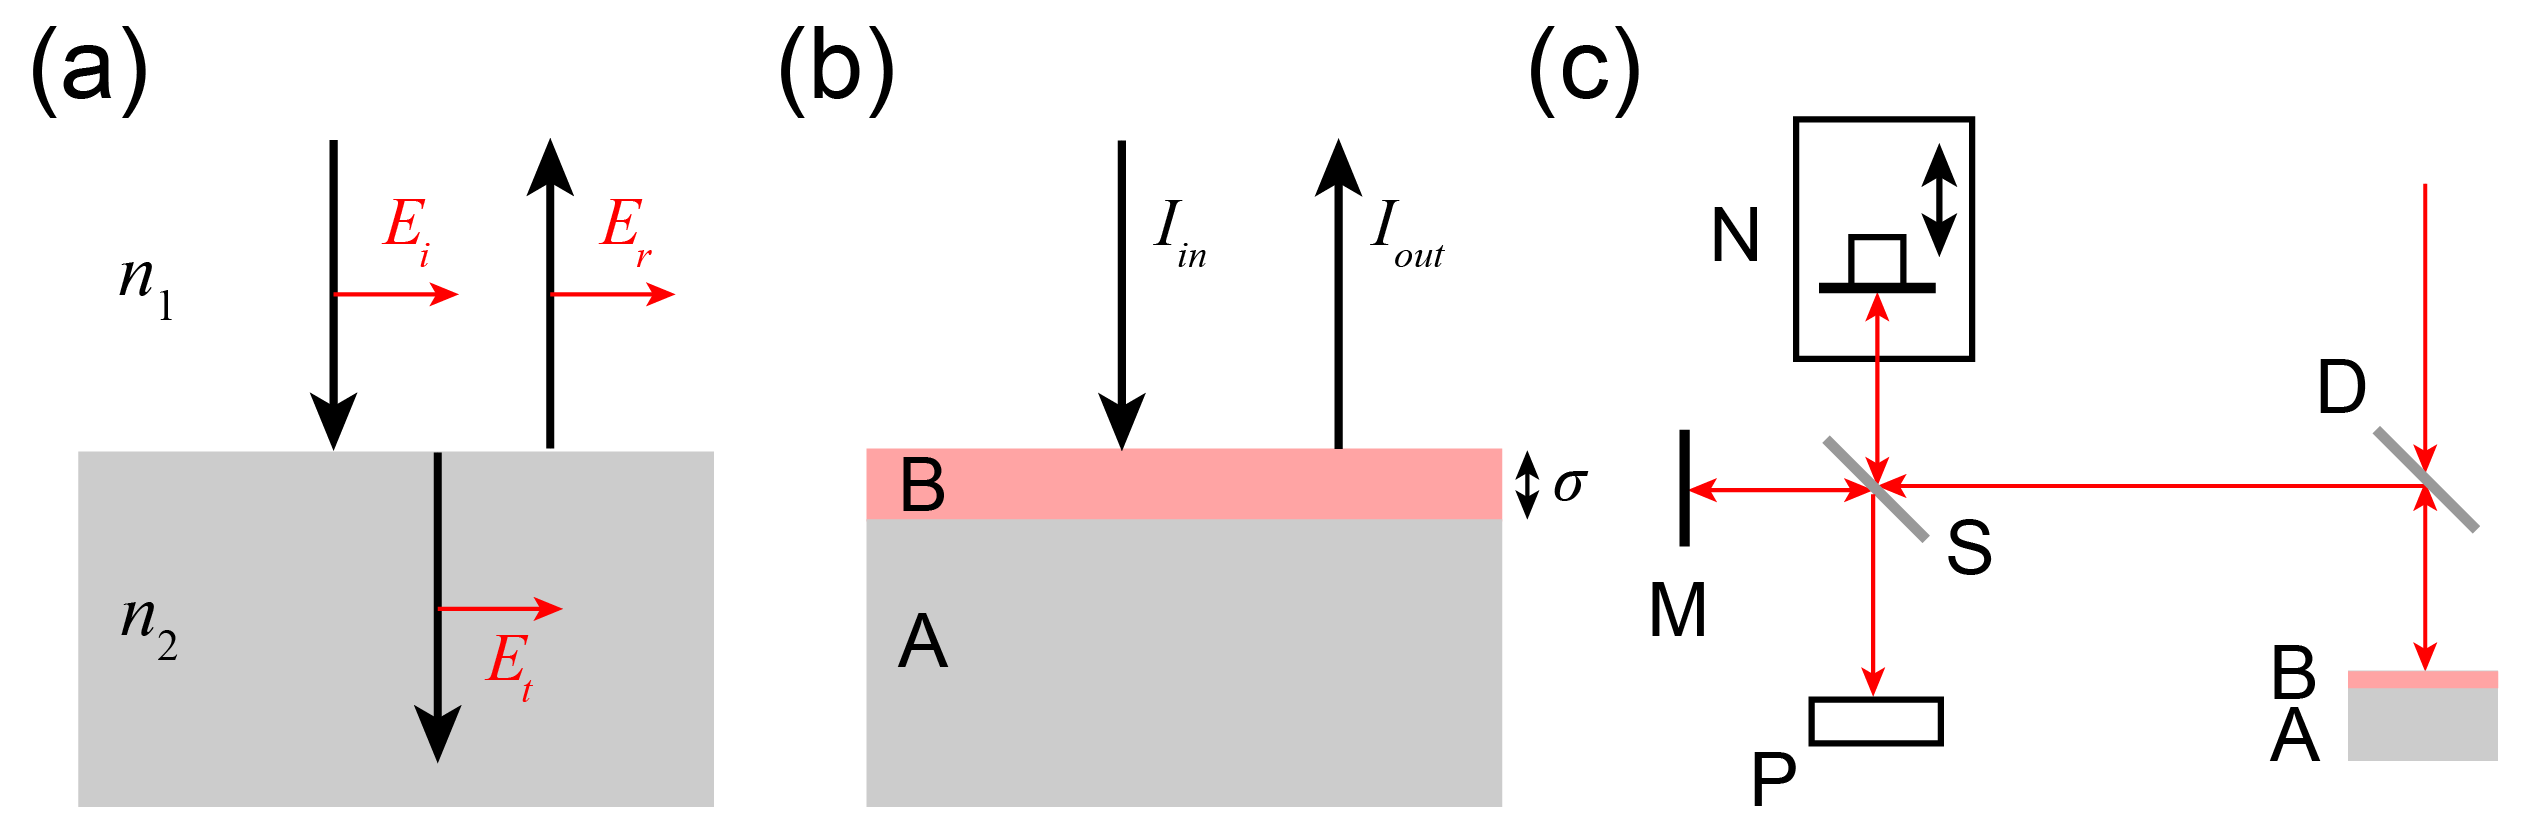
\includegraphics[width=0.95\columnwidth]{5.png}
	\end{figure}
	
	
	
	
	
	\newpage
	\noindent
	\textbf{小孬剧五:此题来自世界一流大学(This Problem Comes From a World-Class University)}
	
	\textit{本题满分$20\ui$分。}
	
	\textit{多年以后,面对不可避免的失业大潮,{\color{white}BECU}将会回想起收到那封信的那个遥远的下午。那时的他坐在荒凉而毫无生气的办公楼里,办公桌上摆着一个巨大的纸质信封。信件来自一个他当年申请时做梦都不敢想的世界著名高等学府,署名是布里渊——是个富有深意的化名。而在他拆开信封之后,信的内容更是令他大吃一惊:}
	
	\begin{quote}
		
		\textit{作为世界名校的高材生,我认为您的所有题目都出得非常不好。例如,学过求导的人只需要计算$a+b/x$关于$x$的偏导就行了,而像我这样不知道$1/x$的导数是什么的人看到您的题目时要考虑的就太多了。我需要专门强调,这一评价绝对不是出于不会做题的私心,而是站在公道的角度反抗邪恶力量对试卷纸、答题纸、草稿纸、评分纸、CASIO FX-991 CN X、以及最后但同样重要的计算机算力的惨无人道的压榨。以上压榨对全球气候变暖的贡献已经到了令人发指的程度。因此,我恳请您调整您的考试范围,并且对所有题目进行彻底的修改。我在信中附上了一些已经成功完成的修改示例。它们的来源并不重要,而且与您的主题不完全相符。但您应当参考这些题目的修改方式,将您的题目也修改得符合世界名校的水平。虽然这些题目我还是不会做,但我认可它们的质量,因为题文中出现的数字我都能数清楚有多少位。}
		
		\textit{\href{https://antimatter-dimensions.fandom.com/wiki/Statistics}{1. }If each antimatter were 1 planck volume, you would have enough to make a proton. If you wrote 3 numbers a second, how many seconds would it take you to write down your antimatter amount? Round to the closest integer.}
		
		\textit{\href{https://projecteuler.net/problem=251}{2. }A pair of positive integers $(a, b)$ is called a Cardano Pair if it satisfies the condition: $\sqrt[3]{a + \sqrt{b}} + \sqrt[3]{a - \sqrt{b}} = 1$. For example, $(2,5)$ is a Cardano Pair. Find how many Cardano Pairs exist such that $a + b \le 999$.}
		
		\textit{\href{https://www.bilibili.com/opus/789540243384565766}{3. }58是初雪八落,初雪八落是0。39是覆夏竹,覆夏竹是X。99是球牡丹,球牡丹是8。27是太阳花,太阳花是4。初雪八落、覆夏竹、球牡丹、太阳花加在一起得到162。请问,X处应该填什么?}
		
		\textit{\href{https://pnku3.pkupuzzle.art/puzzle?key=day3_09}{4. }这道高考作文题看起来像行列式。计算:$(\text{该行列式的值}+13)\mod 26$。}
		
		\textit{\href{https://steamcommunity.com/sharedfiles/filedetails/?id=3267960843}{5. }[2P] Product: Clues represent the product of the distance to the nearest two mines. The numbers that can occur as clues in this rule, in increasing order, are $1,\,\sqrt{2},\,2,\,\sqrt{5},\,\sqrt{8},\,3,\,\sqrt{10},\,\sqrt{13},\,4,\,\sqrt{17},\,\sqrt{X},\,\sqrt{20},\,\cdots$ What is $X$?}
		
		\textit{\href{https://www.bilibili.com/video/BV1iCD2YoEMN}{6. }在异世界的世界顶流大学,有42个人依次排成一排,为DBEWZ、SLCCTD和ZAFNQOG投票竞选猫国总统。初始累加票数为0票,投DBEWZ的话累加票数加1票,投SLCCTD的话累加票数减1票,投ZAFNQOG的话累加票数不变。这42人投完后累加票数为0。请计算这些人可能的投票情况种类,并将结果的个位、十位、百位三个数字相加作为答案。}
		
		\textit{此外,我在这里还向您提供一个经世界名校认可的物理竞赛考试大纲:计算机算力、巴拿赫空间、德国绩点、开四次方、选举投票、波函数、叔本华、猫娘、$\delta$函数、希伯来语、欧拉总计函数、有机合成、失业潮、普朗克尺度、纸质信封、听声辨位、纳维-斯托克斯方程、投资学、实物粒子不能超光速、人工智能、空间群、星座、开普勒天体运动定律、量子色动力学、有限小数与分数的互相转换、手磨原子级平面。}
		
	\end{quote}
	
	\textit{{\color{white}BECU}当然知道自己出的题并不是什么好题,所以在题目的标题里加上了个“孬”字。{\color{white}BECU}当然也知道自己是个藏逼,尤其是在写自己名字的时候。{\color{white}BECU}心里很清楚,这些都是很坏的。{\color{white}BECU}想到这里,甚至开始有些赞同信里说的东西了。{\color{white}BECU}把信纸全部塞回信封,收藏在了办公室柜子的缝隙里。}
	
	\textit{这一象征着不可避免的周期性的物品将永远地留在一个阴暗世界的一个阴暗大楼的一个阴暗角落,而他也一直无法完全原谅自己在过去的日子里的软弱。可以预料这个镜子世界——或蜃景世界——会在他将自己曾经的怯懦和不堪全部遗忘之时被抹去,从世人记忆中根除,离谱中学生物理竞赛中所载一切自永远至永远不会再重复,因为明明早已知晓结局却困于个人无法改变的事物而饱受无谓之苦的轮回不会有第二次机会在大地上出现。}\\
	
	\noindent
	\textbf{题五:真的没有高次谐波吗?(Is There Really No Higher Harmonics?)}
	
	本题满分50分。
	
	有些人认为,如果系统的输入中仅包含一个频率成分(可以认为是正弦波),则系统的输出也会仅有对应的一个频率成分。本题将借助不同的模型讨论这一表述是否正确。
	
	图(a)中的电路由三个线性元件串联而成,分别为电容$C_0$、电感$L_0$、电阻$R_0$。图(b)中的电路也由三个部分串联组成,其中电容和电阻与图(a)相同。感性元件$L'$是非线性元件,其电压--电流关系为
	\begin{equation*}
		u_{L'}(t)=\frac{L_0}{\sqrt{1-(i_{L'}/\iota)^2}}\frac{\ud i_{L'}(t)}{\ud t}
	\end{equation*}
	其中$\iota$为已知量,且$\iota$远大于$i_a(t)$的最大值。
	
	(1)在(a)(b)电路上均加一余弦电压$u(t)=V_0\cos(2\pi f_0 t)$,其中$f_0$和$V_0$已知。在稳定时,图(a)电路中的电流为$i_a(t)$,图(b)中电路的电流为$i_b(t)$。试求$i_a(t)$。再求$i_b(t)-i_a(t)$,保留到$\max[i_a(t)]/\iota$的首阶非零小量。答案中的三角函数可以写成$x\sin(2\pi ft+\theta)$或$x\cos(2\pi ft+\theta)$(其中$\theta$可以含有反三角函数)的形式,不需要进一步展开。
	
	
	在如图(c)所示的电路中,$D_1$和$D_2$是两个理想二极管\footnote{此处,实际的物理情景是器件结构不对称,从而导致正向和反向电压下激发载流子的效率不同。这里简化为两个导通方向不同的理想二极管,物理含义不同但列出的算式相似。}(正向压降为0,反向电流为0)。电阻$R_1=R,R_2=19R,R_3=R$,其中$R$为已知量。在系统上加一周期为$1/f_0$的电压$u(t)$,则流经电阻$R_3$的电流也为周期为$1/f_0$的周期函数$i_c(t)$。根据傅里叶级数理论,$i_c(t)$可以用三角函数展开为
	\begin{align*}
		i_c(t)&=b_0+a_1\sin(2\pi f_0t)+b_1\cos(2\pi f_0t)+a_2\sin(4\pi f_0t)+b_2\cos(4\pi f_0t)+\cdots\\
		&=b_0+c_1\sin(2\pi f_0t+\theta_1)+c_2\sin(4\pi f_0t+\theta_2)+\cdots
	\end{align*}
	其中$c_1,c_2,\cdots$均为非负数,$-\pi\leq\theta_1,\theta_2,\cdots<\pi$。
	
	(2)在(c)电路上加一余弦电压$u(t)=V_0\cos(2\pi f_0 t)$,其中$V_0$为已知量。试求流经电阻$R_3$的电流随时间的变化关系$i_c(t)$,进而求上述展开式中的$b_0$、$c_1$和$c_2$。
	
	(3)在(c)电路上加一带直流偏置的余弦电压$u(t)=V_1\cos(2\pi f_0t)+V_2$,其中$V_1,V_2$在保证$|u(t)|$始终不超过$\upsilon$的情况下可以任意选取。试计算上述条件下$i_c(t)$的展开式中系数$c_1$可取的最大值。表示为$\upsilon/R$乘数值系数的形式,数值结果保留四位有效数字。
	
	提示:对于不相等的非负整数$m,n$,有
	\begin{equation*}
		\int_{-\pi}^{\pi}\sin(mx)\sin(nx)\ud x=0,
		\int_{-\pi}^{\pi}\cos(mx)\cos(nx)\ud x=0
	\end{equation*}
	对于任意的非负整数$m,n$,有
	\begin{equation*}
		\int_{-\pi}^{\pi}\sin(mx)\cos(nx)\ud x=0
	\end{equation*}
	
	
	\begin{figure}[!bh]
	\centering
	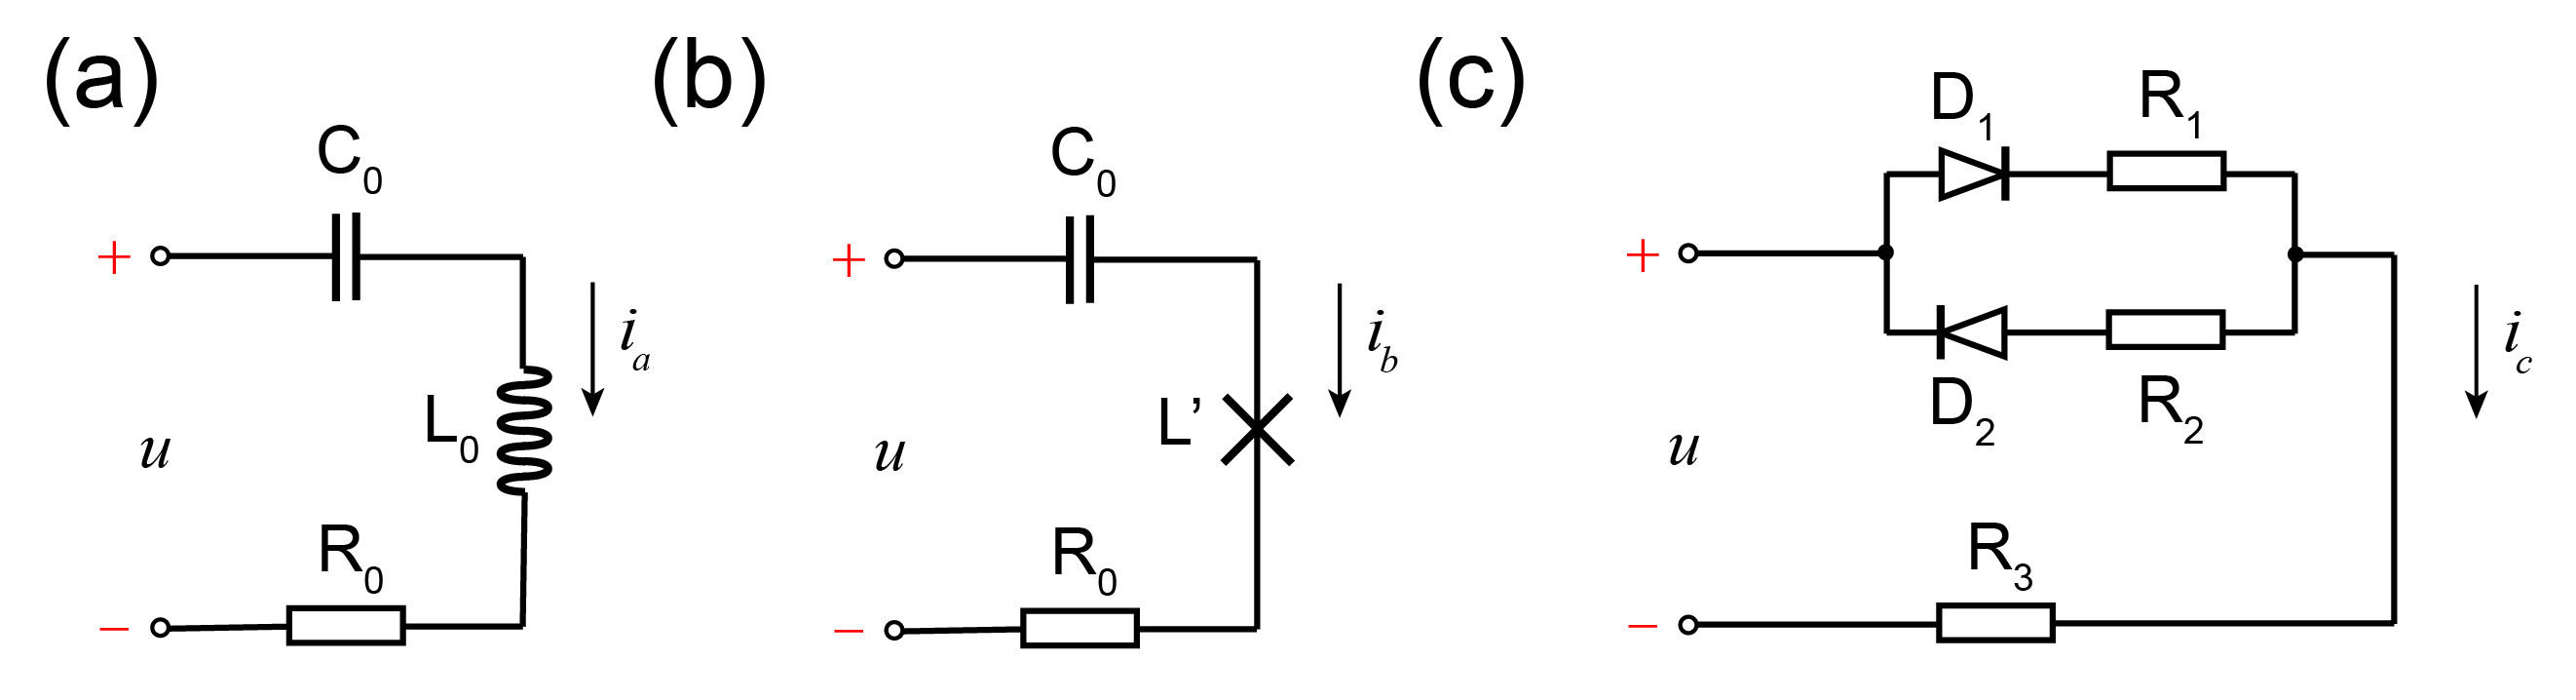
\includegraphics[width=0.92\columnwidth]{6.png}
	\end{figure}
	
	\newpage
	\noindent
	\textbf{小孬剧六:对中学老师来说可能有些幼稚,但对大学教授来说刚刚好(Might be Na\"ive for Middle School Teachers, Must be Just Right for University Professors)}
	
	\textit{本题满分$20\ui$分。}
	
	\textit{说明:“小孬剧六”中的所有信息均对“题六”中的真实分数没有任何帮助。}
	
	\textit{1. $\square\square+\square\square$}
	
	\textit{甲:\fbox{赵凯华},新概念物理教程:光学。高中的时候经常把这里面的事例写进语文作文里。}
	
	\textit{乙:好家伙,学科交叉!}
	
	\textit{甲:结果有一次写了个跟老爹一起站上诺奖领奖台的。}
	
	\textit{乙:厉害啊!然后呢?}
	
	\textit{甲:然后老师说这不是人名,是地名,说我乱编故事。\faMapMarker}
	
	\textit{乙:不能指望语文老师学过物理学史。}
	
	\textit{甲:物理教授也不一定学过啊!}
	
	\textit{乙:这是怎么看出来的?}
	
	\textit{甲:学过物理学史的会不清楚数据选择发表和造假有什么后果?}
	
	\textit{乙:看来你可能学过物理学史,但一定没学过当代物理学。}
	
	\textit{2. $\square\square+\square\square$}
	
	\textit{甲:初中的时候觉得无水硫酸铜和五水硫酸铜这两个词很搞笑。}
	
	\textit{乙:写出来能分清,念出来就分不清了。}
	
	\textit{甲:不过考试的时候也不会让你念,记得一种农药就行了。\faMapMarker}
	
	\textit{乙:语文考试你光会念也没用,得会写。}
	
	\textit{甲:这就导致上了大学还有人把$\nabla$念成delta。}
	
	\textit{乙:你不会念$\nabla$结果怪语文老师,像话吗?}
	
	\textit{3. $\square\square+\square\square$}
	
	\textit{甲:上高中的时候经常粗心,考试的时候扣不该扣的分数。}
	
	\textit{乙:太正常了。}
	
	\textit{甲:最典型的,比如说数学考试,左边1/2、1/8、1/4、2/5什么的,右边0.125、0.25、0.4、0.5什么的,让你连线。结果你少连一根。}
	
	\textit{乙:你这说的真的是高中题目吗?}
	
	\textit{甲:到了大学就反过来了。}
	
	\textit{乙:怎么个反过来法?}
	
	\textit{甲:电子技术课要连电路图,这回线可都连上了。}
	
	\textit{乙:长记性了。}
	
	\textit{甲:结果还是被扣了一半分。}
	
	\textit{乙:这又是怎么一回事呢?}
	
	\textit{甲:说我没用文字描述这线该怎么连。}
	
	\textit{乙:看来是记性还是没长全。这种时候要审题,人家让连线你就连线,让写字你就写字,不能含糊。}
	
	\textit{甲:我一看题目,“为了实现加法器的功能,请将以下部件连接成电路图,句号,图,空两行,下一题”。}
	
	\textit{乙:这就完了?}
	
	\textit{甲:都下一题了,还能没完吗?}
	
	\textit{4. $\square\square+\square\square$}
	
	\textit{甲:上初中的时候家里人想让我当数学家,因为去赌场能赢钱。}
	
	\textit{乙:搞点金融什么的还说得过去,赌博就很搞笑了。}
	
	\textit{甲:那为什么有个算法的名字里面带个赌城?\faMapMarker}
	
	\textit{乙:可能只是想说这玩意的具体输出有一定随机性吧。但它本身是很可靠的,只要上过基础的计算方法课就能写出可以正常运行的代码。}
	
	\textit{甲:那不还是赌博嘛!}
	
	\textit{乙:这我可就不明白了,明明是这么简单的事情。}
	
	\textit{甲:看看有多少人写论文的时候明明不会还硬要装得很懂的样子吧。这可是上再多课都学不到的。}
	
	\textit{5. $\square\square+\square\square$}
	
	\textit{甲:以前上中学的时候经常把卷子剪成一块一块的贴到改错本上。}
	
	\textit{乙:那是,抄一遍题目也挺耽误时间的。}
	
	\textit{甲:如果要是取个极限啊,让剪出来的一片一片的越来越小。}
	
	\textit{乙:那就怎么了呢?}
	
	\textit{甲:那就可以把几张不同卷子上的字贴到一起了。}
	
	\textit{乙:原来是在发明活字乱刷术。}
	
	\textit{甲:这就有一篇呢:“公设:你是李华,你解析几何笔友动点$P$插队变成了首字母,请你帮抛物线的顶点$(a,b)$写一篇谴责,不守规矩的$y=x^2-16x+73$与$y$轴的交点向南方平移$55$得到$c$的纵坐标。已知作文函数$Y(x)$是不得抄袭周期函数,$Y(4x)=\sin(2\pi x)$,$Y(x)$最小的正周期$d$已知。$(33\sqrt{5},0)$是对于$x^2/e^2+y^2/121=f$的一部分焦点,而愤怒的外国人横纵坐标相同是$22\sqrt{3}$,还给出在上面的椭圆。接下来你想要说好,但是副词。然后要透露的操作是接上斯皮尔伯格荧幕的1982年。已经给出的结尾变比较级的时候再字母重复。”}
	
	\textit{乙:你瞅瞅这是$P$吗?人家已经把$P$划掉了改成了$T$了。}
	
	\textit{甲:是我没注意,原来有人在立清解燕。}
	
	\textit{乙:但我还是觉得北大比清华好。}
	
	\textit{甲:这是为什么呢?}
	
	\textit{乙:北大暖气开的比清华早。}
	
	\textit{甲:怎么就扯到暖气上了?}
	
	\textit{乙:一切问题最终都可以由拧暖气阀门来解释。}
	
	\textit{甲:要不你下次见到数学表达式的时候也用拧暖气阀门给解释一下?}\\
	
	\noindent
	\textbf{题六:物理学家有可能理解PID控制吗?(Is it Possible for a Physicist to Understand PID Control?)}
	
	本题满分$60+40\ui$分。
	
	在工业上的很多应用中,需要利用负反馈控制的方法消除系统中出现的噪音。具体而言,我们希望系统中某个物理量的(时间依赖的)实际值$P(t)$与设定值$S$的差异尽可能的小,而为了达成这一点,通常需要让一个控制器实时调节某个可影响系统的变量$U(t)$。该控制器的输入为误差$E(t)=S-P(t)$,同时实时输出一个能让系统尽快回到平衡状态的$U(t)$。
	
	最早的该类控制器是机械式的,基于压缩气体和气缸,其中的关键部件是如图(a)所示的喷管。喷管前有一挡片,实质上是一个力学放大装置。挡片与喷管口之间有距离为$x$的小缝隙。本题考虑的情况都在喷管的线性范围内($x=0$附近),此时喷管上部的压强$p$可以表述为$p=p_0-\beta x$,其中$p_0$和$\beta$为已知正常数。忽略喷管对挡片施加的力。认为喷管的响应关系$p=p_0-\beta x$是即时的,且与气体从喷管中流入和流出的速率无关。
	
	图(b)是一个机械式负反馈控制器的示意图,其主要的机械结构是一个固定在O点的轻质杠杆。A、B两点的上下各通过无摩擦的轻质活塞连接有柱形气缸,其底面积均为$S_0$。在C处的喷管/挡板位于$x=0$的位置时,所有气缸的体积均为$V_0$($V_0/S_0>p_0/\beta$),所有气缸和喷管的轴线均与杠杆垂直。图(c)中有两个限流阀K$_a$和K$_b$,其允许单位时间内通过的气体质量与阀门两端气压差成正比,比例系数分别为$\gamma_a$和$\gamma_b$($\gamma_a<\gamma_b$)。已知A、B、C三点到O的距离分别为$d_1,d_2,d_3$,本问题中涉及的所有喷管/挡板位移大小$|x|\ll d_3$。B点上下两个气缸的气体压强分别为输入控制器的设定值$p_S$和实际值$p_P(t)$,喷管内的压强为控制器的输出$p_U(t)$。设空气是摩尔质量为$\xi$的双原子分子理想气体,理想气体常数为$R_0$。忽略所有管道和限流阀的体积和管壁对流体的阻力。
	
	(1)假设系统已在$p_S=p_P=p_1$的情况下达成长时间的稳定,此时喷管/挡板位于$x=0$处,各气缸中气体的温度均为$T_1$。但在$t=0$时刻,$p_P$从$p_1$突变到$(1+\phi)p_1$(其中$0<\phi\ll 1$)并保持,而$p_S$始终不变。已知$\beta>2p_0^2S_0/(p_1V_0)$,试求在经过该突变杠杆重新达到平衡之后的一瞬间时,系统的输出$P_2=p_U(0^+)$及其变化率$\eta_2=\ud p_U/\ud t|_{t=0^+}$。假设喷管内气体的温度始终为$T_1$。在这极短的时间内,气缸、活塞、限流阀都是绝热的,且其热容可忽略。限流阀对流经气体的阻滞完全转化为热量,并完全被该部分气体吸收。
	
	(2)设A点上下两个气缸内的气体压强分别为$p_a(t)$和$p_b(t)$,改设所有气体的温度均恒定为$T$。假定$\beta\to\infty$,所以$x$始终为$0$。试证明:
	\begin{equation*}
		\frac{p_a(t)}{\gamma_a} -\frac{p_b(t)}{\gamma_b} \propto\int_0^t p_E(t')\ud t'
	\end{equation*}
	其中$p_E(t)=p_S-p_P(t)$。再证明:
	\begin{equation*}
		p_U(t)=K_p p_E(t)+K_i\int_0^t p_E(t')\ud t'+K_d\frac{\ud p_E(t)}{\ud t}
	\end{equation*}
	其中$K_p,K_i,K_d>0$。并给出系数$K_p,K_i,K_d$的表达式。该数学表达式定义了一个PID控制系统,其中各项依次称为比例项P、积分项I、微分项D。试分别解释这三项在负反馈调节中的作用。
	
	后来的PID控制器一般不再是机械式的,而是电子式的,其中的关键部件是如图(c)所示的运算放大器。一个运算放大器有两个输入端$+$和$-$及一个输出端out,以及外接电源S$+$和S$-$。其输出电压与输入电压满足关系$u_O=\alpha(u_+-u_-)$,其中$\alpha$为放大增益,一般而言可以达到或超过$10^5$。这里考虑理想运算放大器的情形,此时认为$\alpha\to\infty$。在这里所涉及的负反馈情形下,理想运算放大器的两个输入端的电压始终相等(即$u_+(t)=u_-(t)$),而电流始终为零(即$i_+(t)=i_-(t)=0$),输出端的输出电压和电流由运算放大器外部所接电路决定。定义所有接地处的电势均为零。
	
	图(d)中给出的元件称为加减法器,其三个输入(in1、in2、in3)中有一个直接连接到$u_E(t)$,另两个分别接入图(e)中两种电路的输出(out)。若将图(e)中两种电路的输入(in)也接到误差$u_E(t)$,则加减法器的输出$u_U(t)$可以实现PID控制。
	
	(3)试将图(d)(e)中的各种部件连接成电路图(图(d)(e)中未画出电源连接口S$+$和S$-$,连线时也不需要连接电源),从而使得该电路的输入$u_E(t)$和输出$u_U(t)$之间满足PID控制器的要求
	\begin{equation*}
		u_U(t)=K_p u_E(t)+K_i\int_0^t u_E(t')\ud t'+K_d\frac{\ud u_E(t)}{\ud t}
	\end{equation*}
	其中$K_p,K_i,K_d>0$。并给出系数$K_p,K_i,K_d$的表达式(用图(d)(e)中标注出的各元件参数表示)。
	
	\begin{figure}[!h]
		\centering
		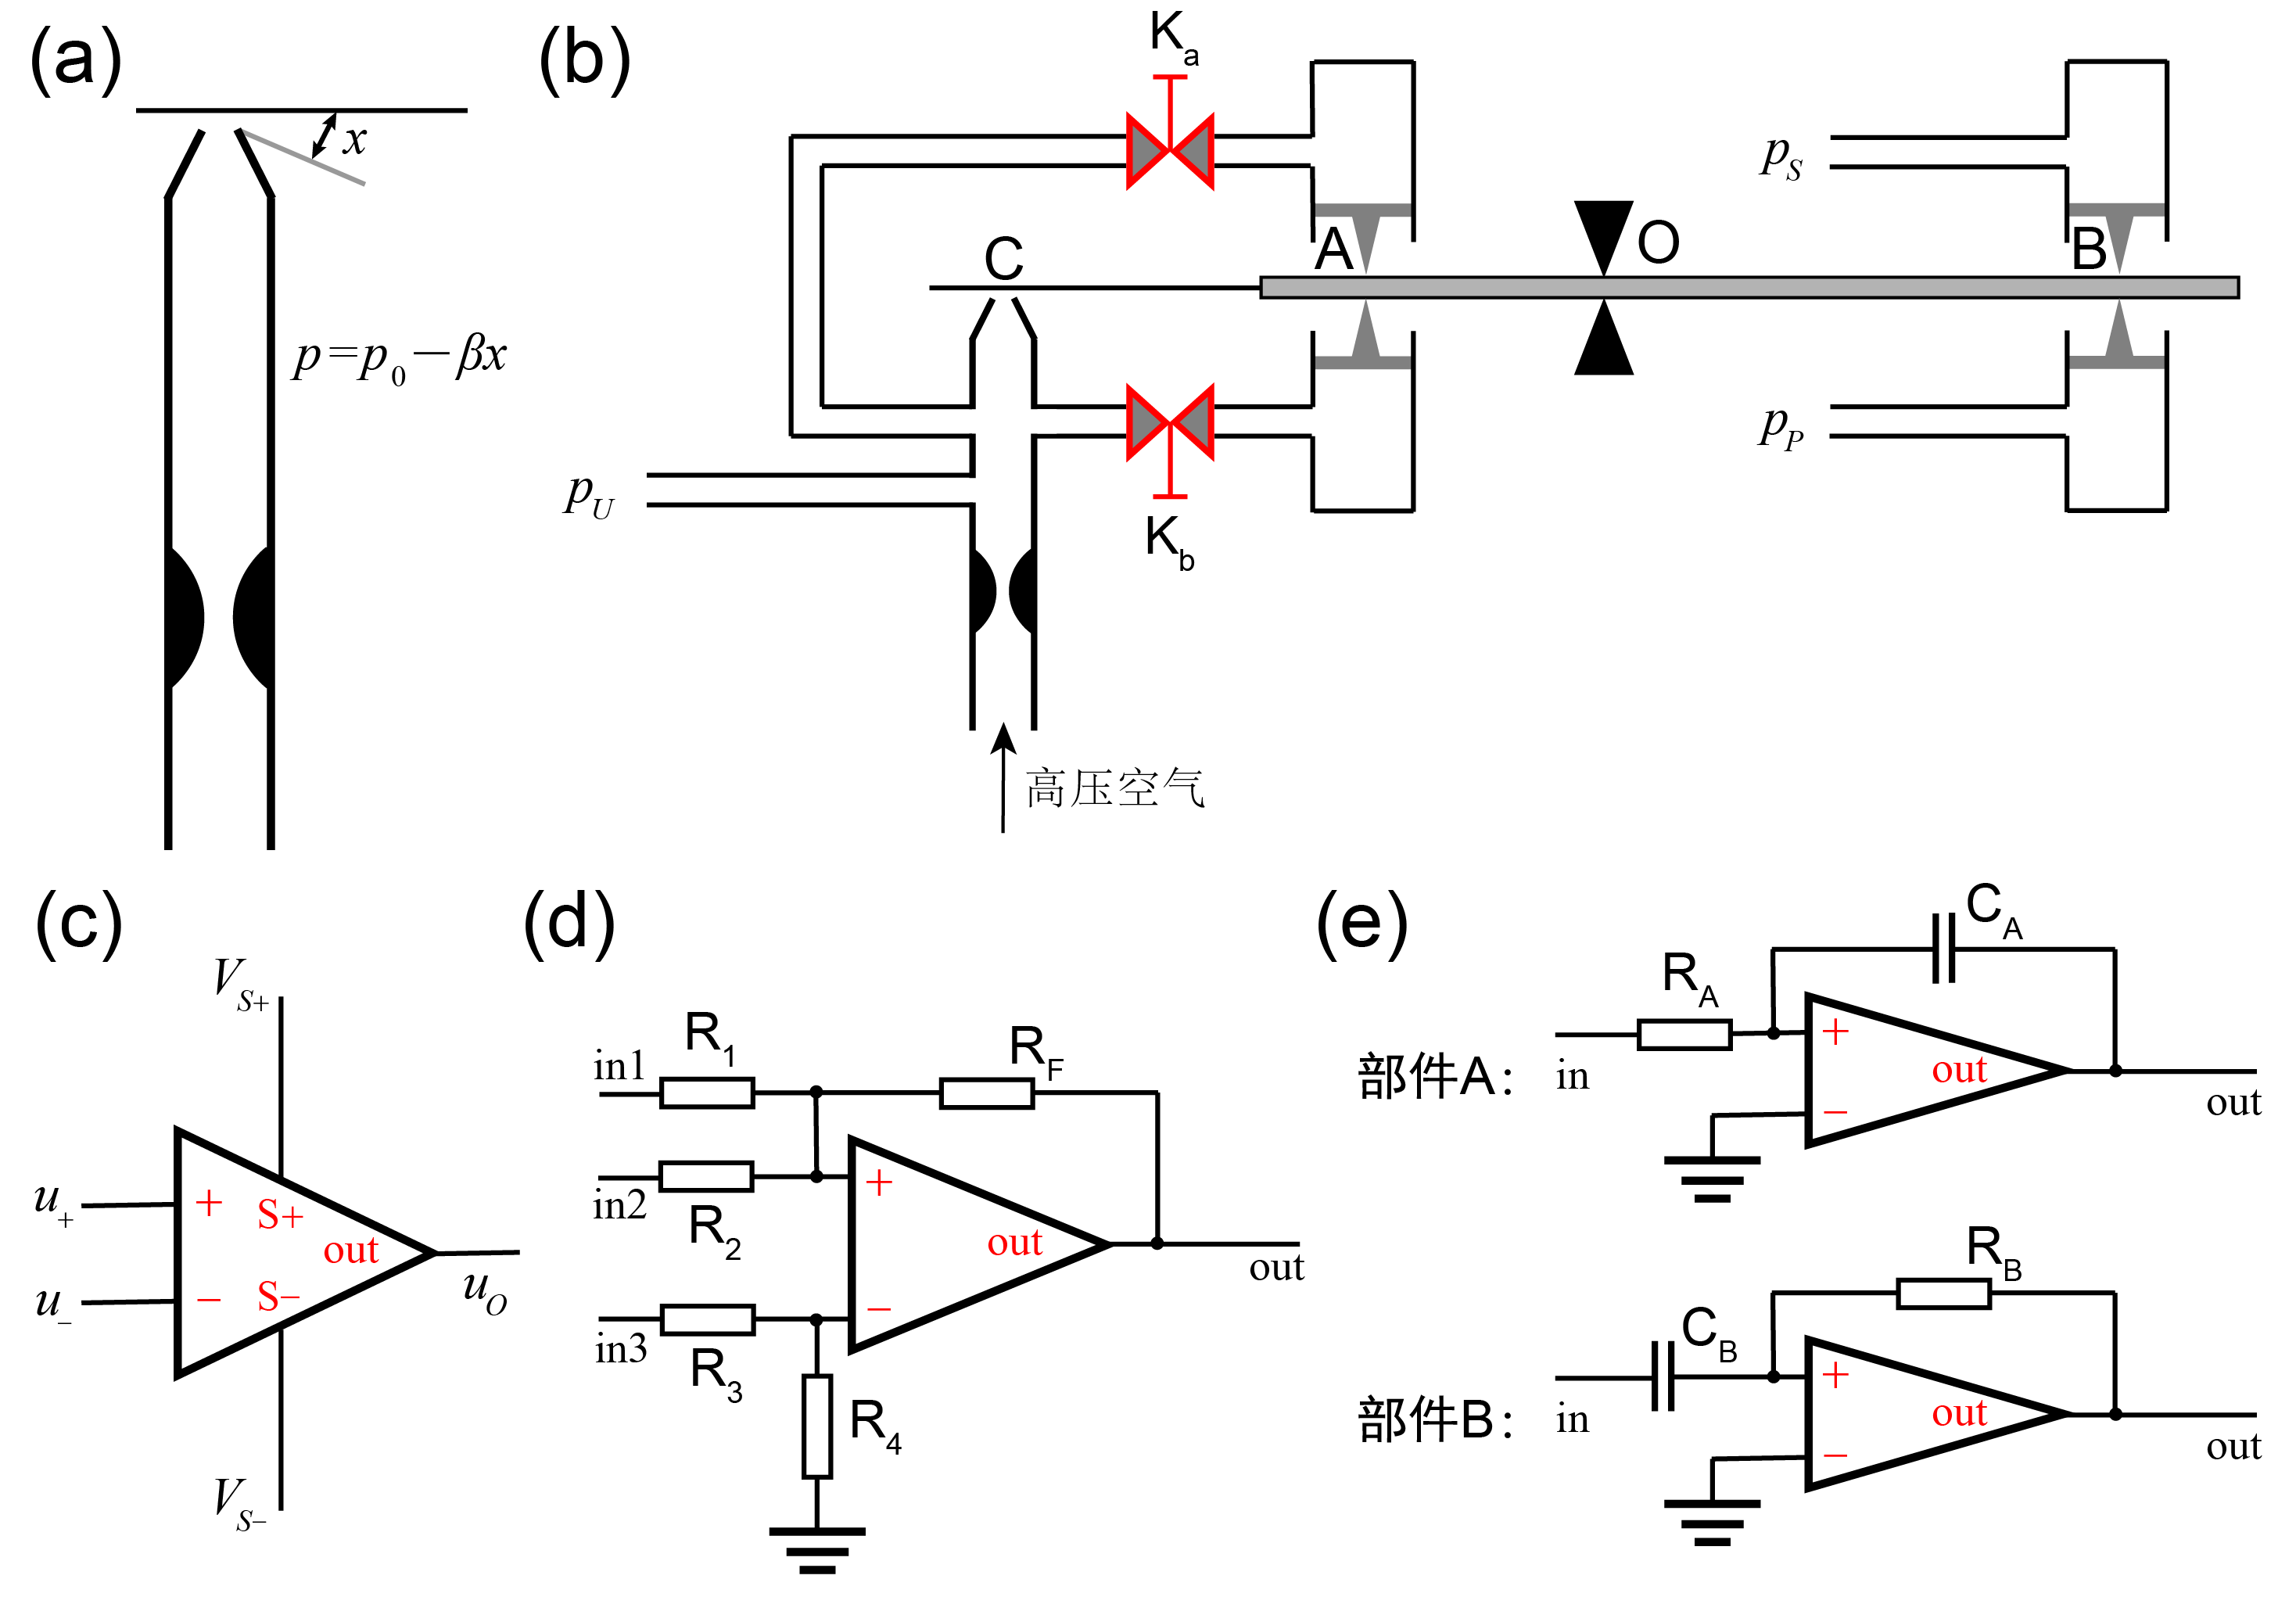
\includegraphics[width=0.99\columnwidth]{7.png}
	\end{figure}
	
	\newpage
	\noindent
	\textbf{结语:重回轨道的交点(Back to the Crosspoints of Tracks)}
	
	\texttt{本题满分$-60\ui$分。}
	
	\texttt{说明:本题题文用仿宋字体写出,这表示本题既属于“小孬剧”部分(楷体),也属于“题”部分(宋体)。本题得分也同时计入上述两部分。本题的解答不需要用到试题版权页、题词页、前言的内容和所有“题”部分的解答,其他内容(包括“题”部分的题文)均可能用到。}
	
	\texttt{\href{https://space.bilibili.com/471367896}{不存在的时间线}里有不存在的地铁线……\href{1,2,3,4,5,6,7,8,9,10,12,...}{不存在的轨道}定义了不存在的交点……借用那些隐藏的联系,将所有真实的抑或虚假的、快要遗忘的抑或即将到来的碎片都重新串起……勾勒出黑色线路的轨迹……}
	
	\texttt{最后,你意识到,在这第十一号线里,还有第十二号、也是最后一号的秘密——只有在这条最漆黑的线路里,你才有回到现实的可能。在那些与现实的交点,在那些你已经看腻了的黑白的名字背后,你可以瞥见五彩斑斓的、另外的颜色——这每一种颜色都意味着另外的可能性。回到现实中去吧,不管迎接你的将是什么,不管你在那里将会做出怎样的选择。}\\
	
	\texttt{答案填写在此处:}\_\_\_\_\_\_\_\_\_\_\_\_\texttt{(不区分大小写,不需要空格)}\\
	
	\begin{figure}[!h]
		\centering
		\includegraphics[width=0.99\columnwidth]{11A.png}
	\end{figure}
	
	\begin{figure}[!h]
	\centering
	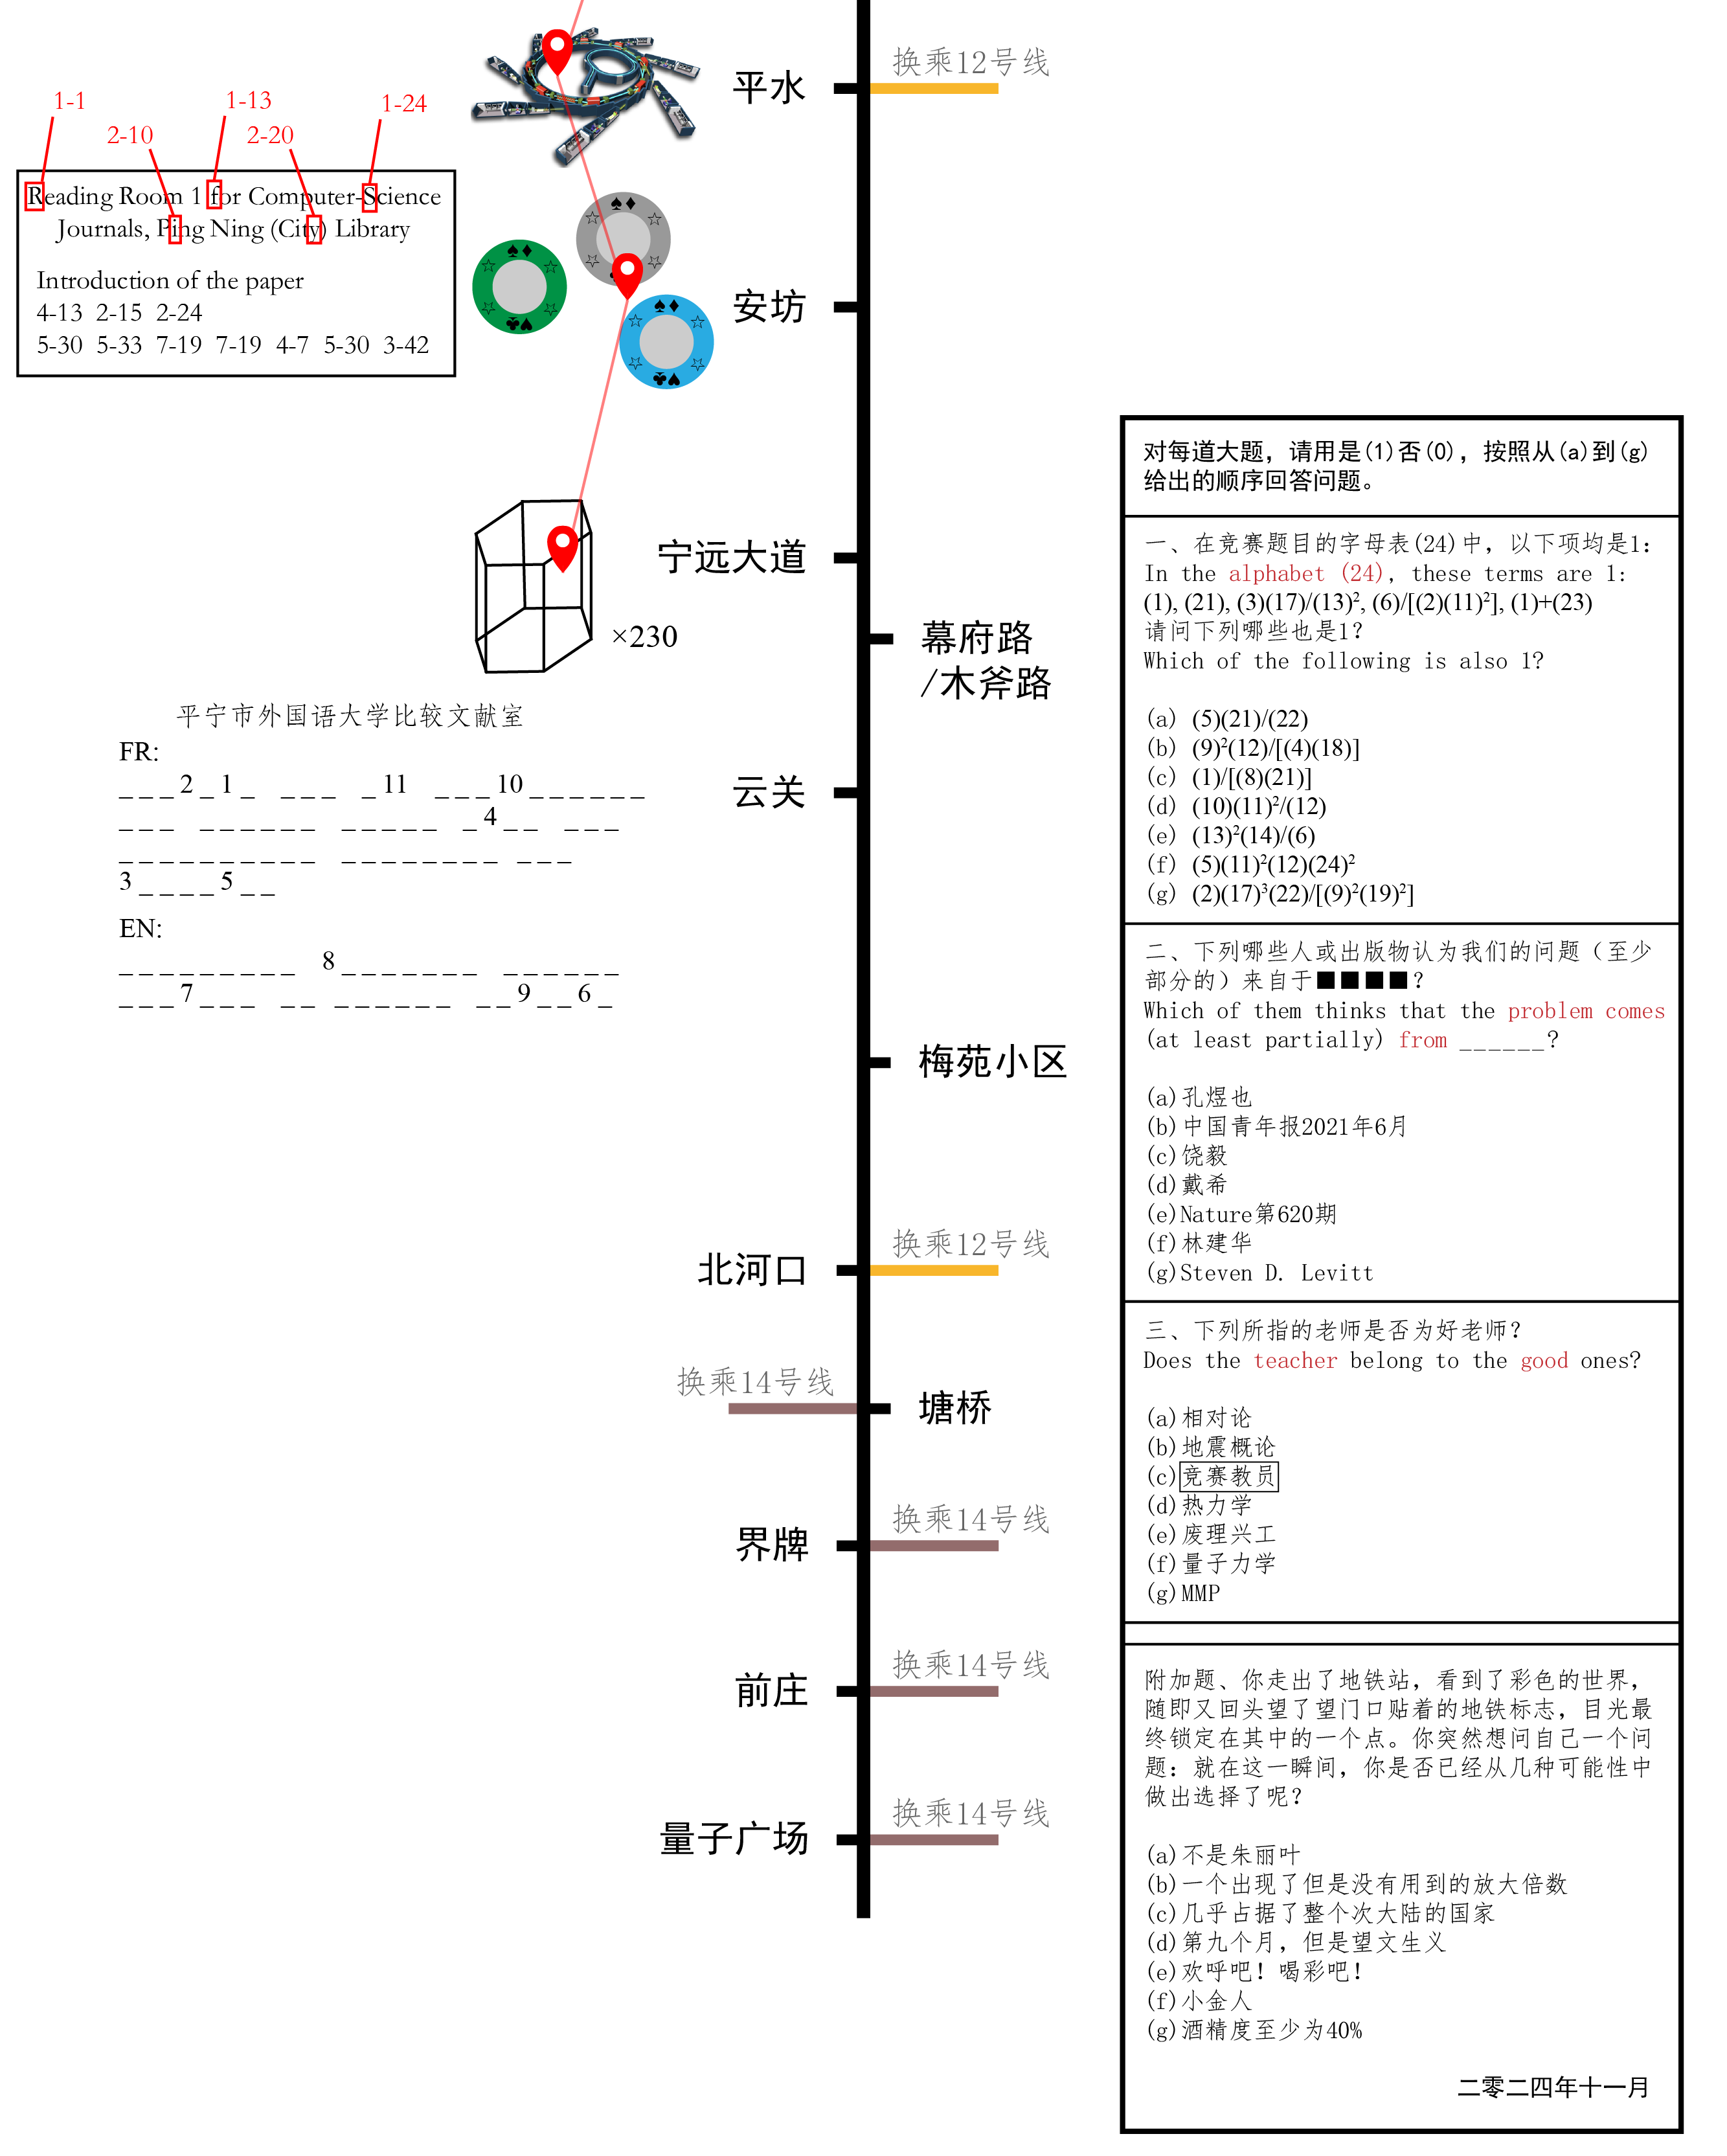
\includegraphics[width=0.99\columnwidth]{11B.png}
	\end{figure}
	
	\newpage
	
	\textit{提示:本文档的图片版信息不全,强烈建议在作答“小孬剧”和“结语”时采用PDF版本。“前言”中已经提及解答部分谜题需要一定的数理基础,不建议在没有对应知识水平的情况下尝试。如果你对“小孬剧”和“结语”的形式完全不熟悉,或者发现自己看不懂一些似乎是很基本的记号,下面有一些白色的字,你可以将之复制粘贴出来。}
		
	\footnotesize{\color{white}\textit{(a)你可能需要对凯撒密码、莫尔斯电码、ASCII码、猪圈密码、A1Z26、倒序、NATO字母表等加密方式有基本的了解。(b)当下划线与数字同时出现时,一般每个下划线或每个数字各代表一个字母,而数字表示对应字母在答案中的位置。(c)孤立的一个或多个数字可能代表答案有几个字母,或者需要提取该答案中的第几个字母。(d)计算工具和搜索引擎可以起到很好的辅助作用。(e)“前言”中提到最终答案是一个有意义的英文词组,你可以利用这一点。}}
	
	
	
	
	
	
	
\end{document}